% ============================================================
%  يُترجَم بـ XeLaTeX  (في Overleaf: Menu → Compiler → XeLaTeX)
%  الخط: Amiri (متوفر في Overleaf، أو حمّله من github.com/aliftype/amiri)
% ============================================================
\documentclass[12pt,a4paper]{article}
\usepackage[a4paper,margin=1.7cm,top=2.3cm,bottom=2.9cm,headheight=15pt,footskip=1.5cm]{geometry}
\usepackage{amsmath,amssymb}
\usepackage{icomma}
\usepackage[english,bidi=default,layout=lists]{babel}
\babelprovide[import,main]{arabic}
\babelfont{rm}[Scale=1.08]{Amiri}
\babelfont{sf}[Scale=1.08]{Amiri}
\usepackage[most]{tcolorbox}
\usepackage{tikz}
\usetikzlibrary{arrows.meta,calc,shadings}
\usepackage{array}
\usepackage{colortbl}
\usepackage{fancyhdr}
\usepackage{titlesec}
\usepackage{enumitem}
\usepackage{collcell}
\usepackage{needspace}
\usepackage{etoolbox}
\newcolumntype{C}{>{\collectcell\ar}c<{\endcollectcell}}
\pretocmd{\section}{\Needspace{15\baselineskip}}{}{}
\pretocmd{\subsection}{\Needspace{11\baselineskip}}{}{}

\definecolor{cDef}{HTML}{1F4E9C}
\definecolor{cThm}{HTML}{B3261E}
\definecolor{cRem}{HTML}{2E7D32}
\definecolor{cEx}{HTML}{C76B00}
\definecolor{cMeth}{HTML}{6A1B9A}
\definecolor{cSol}{HTML}{00695C}
\definecolor{cSec}{HTML}{1F3A68}

\titleformat{\section}{\Large\bfseries\color{cSec}}{\thesection.}{0.6em}{}[{\color{cSec!60}\titlerule[1pt]}]
\titleformat{\subsection}{\large\bfseries\color{cThm!85!black}}{\thesubsection.}{0.5em}{}
\titlespacing*{\section}{0pt}{14pt}{8pt}
\titlespacing*{\subsection}{0pt}{10pt}{5pt}
\setlength{\parindent}{0pt}
\setlength{\parskip}{4pt}
\setlist{itemsep=2pt,topsep=3pt}

\newtcolorbox{arbox}[3][]{enhanced,
  colback=#2!5,colframe=#2!80!black,arc=2mm,boxrule=0.8pt,
  left=6pt,right=6pt,top=8pt,bottom=5pt,
  fonttitle=\bfseries,coltitle=white,
  title={\foreignlanguage{arabic}{#3}},
  attach boxed title to top right={xshift=-5mm,yshift=-3mm},
  boxed title style={colback=#2!80!black,arc=1.5mm,boxrule=0pt},
  before upper={\selectlanguage{arabic}},
  before skip=8pt,after skip=8pt,breakable,#1}
\newenvironment{BOX}[2]{\begin{otherlanguage}{english}\begin{arbox}{#1}{#2}}{\end{arbox}\end{otherlanguage}}
\newenvironment{tarif}[1][تعريف]{\begin{BOX}{cDef}{#1}}{\end{BOX}}
\newenvironment{khassia}[1][خاصية]{\begin{BOX}{cThm}{#1}}{\end{BOX}}
\newenvironment{molahada}[1][ملاحظة]{\begin{BOX}{cRem}{#1}}{\end{BOX}}
\newenvironment{mithal}[1][مثال]{\begin{BOX}{cEx}{#1}}{\end{BOX}}
\newenvironment{tariqa}[1][طريقة]{\begin{BOX}{cMeth}{#1}}{\end{BOX}}

\newcounter{exo}
\newenvironment{tamrin}[1]{\stepcounter{exo}\begin{BOX}{cSec}{التمرين \theexo: #1}}{\end{BOX}}
\newenvironment{hal}{\Needspace{12\baselineskip}\begin{otherlanguage}{english}\begin{arbox}[breakable]{cSol}{حل التمرين \theexo}}{\end{arbox}\end{otherlanguage}}

\newenvironment{LTR}{\begin{otherlanguage}{english}}{\end{otherlanguage}}
\newcommand{\ar}[1]{\foreignlanguage{arabic}{#1}}

\renewcommand{\dots}{\mathinner{\ldotp\ldotp\ldotp}}
\renewcommand{\ldots}{\mathinner{\ldotp\ldotp\ldotp}}
\renewcommand{\cdots}{\mathinner{\cdotp\cdotp\cdotp}}
\newcommand{\N}{\mathbb{N}}
\newcommand{\Z}{\mathbb{Z}}
\newcommand{\D}{\mathbb{D}}
\newcommand{\Q}{\mathbb{Q}}
\newcommand{\R}{\mathbb{R}}
\newcommand{\pgcd}{\operatorname{PGCD}}
\newcommand{\ppcm}{\operatorname{PPCM}}

% \NLseg{a}{b}{[}{]} ; \NLright{a}{[} ; \NLleft{b}{]}  (interval on a number line)
\newcommand{\NLseg}[4]{\begin{LTR}\begin{tikzpicture}[baseline=-0.6ex]
 \draw[-{Stealth[length=2mm]},gray!70](0,0)--(3.4,0);
 \draw[line width=2pt,cThm!80!black](0.7,0)--(2.7,0);
 \node[cThm!80!black,font=\LARGE] at (0.7,0){$#3$};
 \node[cThm!80!black,font=\LARGE] at (2.7,0){$#4$};
 \node[below=3pt,font=\footnotesize] at (0.7,0){$#1$};
 \node[below=3pt,font=\footnotesize] at (2.7,0){$#2$};
\end{tikzpicture}\end{LTR}}
\newcommand{\NLright}[2]{\begin{LTR}\begin{tikzpicture}[baseline=-0.6ex]
 \draw[-{Stealth[length=2mm]},gray!70](0,0)--(3.4,0);
 \draw[line width=2pt,cThm!80!black](1.3,0)--(3.3,0);
 \node[cThm!80!black,font=\LARGE] at (1.3,0){$#2$};
 \node[below=3pt,font=\footnotesize] at (1.3,0){$#1$};
\end{tikzpicture}\end{LTR}}
\newcommand{\NLleft}[2]{\begin{LTR}\begin{tikzpicture}[baseline=-0.6ex]
 \draw[-{Stealth[length=2mm]},gray!70](0,0)--(3.4,0);
 \draw[line width=2pt,cThm!80!black](0.05,0)--(2.1,0);
 \node[cThm!80!black,font=\LARGE] at (2.1,0){$#2$};
 \node[below=3pt,font=\footnotesize] at (2.1,0){$#1$};
\end{tikzpicture}\end{LTR}}

% ---------- social-media icons (pure TikZ) ----------
\definecolor{cFB}{HTML}{1877F2}
\definecolor{cTG}{HTML}{229ED9}
\definecolor{cIG1}{HTML}{FEDA75}
\definecolor{cIG2}{HTML}{D62976}
\definecolor{cIG3}{HTML}{4F5BD5}
\newcommand{\fbicon}{\begin{LTR}\begin{tikzpicture}[baseline=-0.75ex,x=1em,y=1em]
 \fill[cFB] (0,0) circle (0.55);
 \node[white,inner sep=0,font=\usefont{TU}{lmss}{bx}{n}\small] at (0.04,-0.02) {f};
\end{tikzpicture}\end{LTR}}
\newcommand{\igicon}{\begin{LTR}
\begin{tikzpicture}[baseline=-0.75ex,x=1em,y=1em]
 \shade[lower left=cIG1,lower right=cIG2,upper left=cIG2,upper right=cIG3,rounded corners=0.28em] (-0.55,-0.55) rectangle (0.55,0.55);
 \draw[white,line width=0.09em,rounded corners=0.18em] (-0.36,-0.36) rectangle (0.36,0.36);
 \draw[white,line width=0.09em] (0,0) circle (0.17);
 \fill[white] (0.22,0.22) circle (0.05);
\end{tikzpicture}\end{LTR}}
\newcommand{\tgicon}{\begin{LTR}
\begin{tikzpicture}[baseline=-0.75ex,x=1em,y=1em]
 \fill[cTG] (0,0) circle (0.55);
 \fill[white] (-0.33,0.0) -- (0.32,0.27) -- (0.2,-0.3) -- (0.0,-0.15) -- (-0.08,-0.28) -- (-0.08,-0.08) -- cycle;
 \fill[cTG!70!black] (-0.08,-0.08) -- (0.25,0.2) -- (0.0,-0.15) -- (-0.08,-0.28) -- cycle;
\end{tikzpicture}\end{LTR}}
% page number: black box, white two-digit number, at the right of the social row
\newcommand{\PageBox}{\begin{LTR}\tikz[baseline=(p.base)]\node[fill=black,text=white,inner sep=2.5pt,minimum width=1.6em,minimum height=1.3em,font=\usefont{TU}{lmss}{bx}{n}\small](p){\ifnum\value{page}<10 0\fi\arabic{page}};\end{LTR}}
% visual left-to-right order: Telegram | Instagram | Facebook | page box
\newcommand{\SocialRow}{\begin{otherlanguage}{english}%
 \ar{\textbf{الأستاذ سوايسية هشام للرياضيات}}\ \tgicon\hfill
 \textbf{prof\_hicham\_math}\ \igicon\hfill
 \ar{\textbf{الأستاذ سوايسية هشام للرياضيات}}\ \fbicon\hspace{2.2em}\PageBox\end{otherlanguage}}

\pagestyle{fancy}
\fancyhf{}
\renewcommand{\headrulewidth}{0.6pt}
\renewcommand{\footrulewidth}{0.4pt}
% \SetHeader{right head: document title}{left head: level -- stream}
\newcommand{\SetHeader}[2]{%
 \fancyhead[C]{\parbox{\textwidth}{\ar{#1\hfill #2}}}%
 \fancyfoot[C]{\parbox{\textwidth}{\small\SocialRow}}}
\usepackage{tkz-tab}
\usepackage{multicol}
% variation / sign table (LTR)
\newenvironment{TAB}{\par\begin{center}\begin{LTR}\begin{tikzpicture}[scale=0.95,every node/.style={font=\small}]}{\end{tikzpicture}\end{LTR}\end{center}}
% grid + axes, clipped: \begin{GR}{xmin}{xmax}{ymin}{ymax}{unit cm}
\newenvironment{GR}[5]{\par\begin{center}\begin{LTR}\begin{tikzpicture}[x=#5cm,y=#5cm,font=\footnotesize]
 \draw[gray!25,very thin] (#1,#3) grid (#2,#4);
 \draw[-{Stealth[length=2mm]}] (#1,0)--(#2+0.3,0) node[below left]{$x$};
 \draw[-{Stealth[length=2mm]}] (0,#3)--(0,#4+0.3) node[below left]{$y$};
 \node[below left] at (0,0){$O$};
 \begin{scope}\clip (#1,#3) rectangle (#2,#4);}
{\end{scope}\end{tikzpicture}\end{LTR}\end{center}}
\newcommand{\Ticks}[2]{\foreach \t in {#1} \node[below,font=\scriptsize] at (\t,0){$\t$}; \foreach \t in {#2} \node[left,font=\scriptsize] at (0,\t){$\t$};}
\newcommand{\bx}[1]{\ensuremath{\colorbox{cDef!12}{$\displaystyle #1$}}}
\newcommand{\TwoCol}[4]{\par\begin{LTR}\noindent\begin{minipage}[t]{#1\textwidth}\selectlanguage{arabic}#2\end{minipage}\hfill\begin{minipage}[t]{#3\textwidth}\selectlanguage{arabic}#4\end{minipage}\end{LTR}\par}
\newcommand{\RL}[4]{\TwoCol{#3}{#4}{#1}{#2}}  % \RL{w1}{right content}{w2}{left content}
\newcommand{\ok}{$\textcolor{cRem}{\checkmark}$}
\newcommand{\limn}{\displaystyle\lim_{n\to+\infty}}
% sub-questions, each on its own line
\newenvironment{sq}{\begin{itemize}[leftmargin=2.4em,itemsep=3pt]}{\end{itemize}}
\newcommand{\qa}{\item[(أ)]}\newcommand{\qb}{\item[(ب)]}\newcommand{\qc}{\item[(جـ)]}\newcommand{\qd}{\item[(د)]}\newcommand{\qe}{\item[(هـ)]}
\newcommand{\pa}{\par\smallskip\textbf{(أ)} }\newcommand{\pb}{\par\smallskip\textbf{(ب)} }\newcommand{\pc}{\par\smallskip\textbf{(جـ)} }\newcommand{\pd}{\par\smallskip\textbf{(د)} }\newcommand{\pe}{\par\smallskip\textbf{(هـ)} }
\newcommand{\QQ}[1]{\par\smallskip\textbf{#1.} }
\newenvironment{tmr}{\stepcounter{exo}\begin{BOX}{cSec}{تمرين محلول \theexo}}{\end{BOX}}
\newcommand{\ABC}[3]{\\[2pt]\begin{tabular}{p{0.28\textwidth}p{0.28\textwidth}p{0.28\textwidth}}(جـ) \ #3 & (ب) \ #2 & (أ) \ #1\end{tabular}}
\pretocmd{\section}{\Needspace{24\baselineskip}}{}{}
\newtcbox{\bxtbox}{on line,colback=cDef!12,colframe=cDef!12,boxrule=0pt,arc=1pt,boxsep=0pt,left=2pt,right=2pt,top=1pt,bottom=1pt}
\newcommand{\bxt}[1]{\foreignlanguage{english}{\bxtbox{\ar{#1}}}}
\SetHeader{\small\bfseries\color{cSec}تمارين تجريبية: الدالة اللوغاريتمية}{\small\color{cSec}السنة الثالثة ثانوي -- الشعب العلمية}
\newenvironment{FIG}{\par\begin{center}\begin{LTR}}{\end{LTR}\end{center}}
\begin{document}
\begin{LTR}
\begin{tcolorbox}[enhanced,colback=cSec,colframe=cSec,arc=3mm,halign=center,boxrule=0pt,top=12pt,bottom=12pt,before upper={\selectlanguage{arabic}}]
{\color{white}\fontsize{26}{32}\selectfont\bfseries تمارين تجريبية في الدالة اللوغاريتمية}\\[8pt]
{\color{white}\large تمارين متدرجة مع الحلول المفصلة خطوة بخطوة}\\[5pt]
{\color{white}\large السنة الثالثة ثانوي -- الشعب العلمية}
\end{tcolorbox}
\end{LTR}
\section{مجموعة التعريف والتبسيط}

% ------------------------------------------------------------------
\begin{tamrin}{مجموعة تعريف دالة}
عيّن مجموعة تعريف كل دالة من الدوال التالية:
\QQ{1} $f_1(x)=\ln(2x-4)$
\QQ{2} $f_2(x)=\ln(3-x)+\ln(x+1)$
\QQ{3} $f_3(x)=\ln\left(\dfrac{x-1}{x+2}\right)$
\QQ{4} $f_4(x)=\ln\left|x^2-1\right|$
\QQ{5} $f_5(x)=\dfrac{x}{\ln x}$
\QQ{6} $f_6(x)=\dfrac{1}{1-\ln x}$
\QQ{7} $f_7(x)=\ln\left(e^{x}-1\right)$
\end{tamrin}
\begin{hal}
\textbf{تذكير:} الدالة $x\mapsto \ln\big(u(x)\big)$ معرفة من أجل كل $x$ يحقق $u(x)>0$، والدالة $x\mapsto \ln|u(x)|$ معرفة من أجل كل $x$ يحقق $u(x)\neq 0$.

\QQ{1} $f_1$ معرفة معناه $2x-4>0$ أي $x>2$. إذن \bx{D_{f_1}=\left]2;+\infty\right[}

\QQ{2} $f_2$ معرفة معناه $3-x>0$ و $x+1>0$، أي $x<3$ و $x>-1$.
إذن \bx{D_{f_2}=\left]-1;3\right[}

\QQ{3} $f_3$ معرفة معناه $x\neq -2$ و $\dfrac{x-1}{x+2}>0$. ندرس إشارة الحاصل:
\begin{TAB}
\tkzTabInit[lgt=2.6,espcl=2]{$x$/0.8,$x-1$/0.8,$x+2$/0.8,$\dfrac{x-1}{x+2}$/1.1}{$-\infty$,$-2$,$1$,$+\infty$}
\tkzTabLine{,-,t,-,z,+,}
\tkzTabLine{,-,z,+,t,+,}
\tkzTabLine{,+,d,-,z,+,}
\end{TAB}
إذن \bx{D_{f_3}=\left]-\infty;-2\right[\cup\left]1;+\infty\right[}

\QQ{4} $f_4$ معرفة معناه $x^2-1\neq 0$ أي $x\neq 1$ و $x\neq -1$.
إذن \bx{D_{f_4}=\R-\{-1;1\}}

\QQ{5} $f_5$ معرفة معناه $x>0$ (لكي يكون $\ln x$ معرفا) و $\ln x\neq 0$ أي $x\neq 1$.
إذن \bx{D_{f_5}=\left]0;1\right[\cup\left]1;+\infty\right[}

\QQ{6} $f_6$ معرفة معناه $x>0$ و $1-\ln x\neq 0$، أي $\ln x\neq 1$ ومنه $x\neq e$.
إذن \bx{D_{f_6}=\left]0;e\right[\cup\left]e;+\infty\right[}

\QQ{7} $f_7$ معرفة معناه $e^{x}-1>0$ أي $e^{x}>e^{0}$، ولأن الدالة الأسية متزايدة تماما على $\R$ فإن $x>0$.
إذن \bx{D_{f_7}=\left]0;+\infty\right[}
\end{hal}

% ------------------------------------------------------------------
\begin{tamrin}{تبسيط عبارات}
\QQ{1} اكتب بدلالة $\ln 2$ و $\ln 3$ كلا من الأعداد:
\begin{sq}
\qa $A=\ln 8+\ln 2-\ln 4$
\qb $B=\ln 72$
\qc $C=\ln\sqrt{12}$
\qd $D=\ln\dfrac{4}{9}$
\qe $E=\ln 27-2\ln 3+\ln\dfrac{1}{9}$
\end{sq}
\QQ{2} بسّط ما يلي:
\begin{sq}
\qa $F=\ln\sqrt{e}+\ln\dfrac{1}{e^{2}}-\ln\left(e^{3}\right)$
\qb $G=\ln\left(\sqrt{3}+\sqrt{2}\right)+\ln\left(\sqrt{3}-\sqrt{2}\right)$
\qc $H=e^{2\ln 3}-\ln\left(e^{-2}\right)$
\end{sq}
\QQ{3} بيّن أنه من أجل كل عدد حقيقي $x$: \ $\ln\left(e^{x}+1\right)-x=\ln\left(1+e^{-x}\right)$.
\end{tamrin}
\begin{hal}
نستعمل الخواص: من أجل $a>0$ و $b>0$ و $n\in\Z$:
$\ln(ab)=\ln a+\ln b$، \ $\ln\dfrac{a}{b}=\ln a-\ln b$، \ $\ln a^{n}=n\ln a$، \ $\ln\sqrt{a}=\dfrac12\ln a$، \ $\ln e^{x}=x$ و $e^{\ln a}=a$.

\QQ{1}
\pa $A=\ln 2^{3}+\ln 2-\ln 2^{2}=3\ln 2+\ln 2-2\ln 2$ إذن \bx{A=2\ln 2}
\pb $72=8\times 9=2^{3}\times 3^{2}$ ومنه $B=\ln 2^{3}+\ln 3^{2}$ إذن \bx{B=3\ln 2+2\ln 3}
\pc $12=2^{2}\times 3$ ومنه $C=\dfrac12\ln 12=\dfrac12\left(2\ln 2+\ln 3\right)$ إذن \bx{C=\ln 2+\dfrac12\ln 3}
\pd $D=\ln 4-\ln 9=\ln 2^{2}-\ln 3^{2}$ إذن \bx{D=2\ln 2-2\ln 3}
\pe $E=\ln 3^{3}-2\ln 3-\ln 9=3\ln 3-2\ln 3-2\ln 3$ إذن \bx{E=-\ln 3}

\QQ{2}
\pa $\ln\sqrt e=\ln e^{\frac12}=\dfrac12$ و $\ln\dfrac{1}{e^{2}}=\ln e^{-2}=-2$ و $\ln e^{3}=3$، ومنه
$F=\dfrac12-2-3$ إذن \bx{F=-\dfrac92}
\pb العددان $\sqrt3+\sqrt2$ و $\sqrt3-\sqrt2$ موجبان تماما، إذن:
\[G=\ln\Big[\left(\sqrt3+\sqrt2\right)\left(\sqrt3-\sqrt2\right)\Big]=\ln\left(3-2\right)=\ln 1\]
إذن \bx{G=0}
\pc $e^{2\ln 3}=e^{\ln 3^{2}}=e^{\ln 9}=9$ و $\ln e^{-2}=-2$، ومنه $H=9-(-2)$ إذن \bx{H=11}

\QQ{3} من أجل كل عدد حقيقي $x$: $e^{x}+1>0$ و $1+e^{-x}>0$، ولدينا $x=\ln e^{x}$، إذن:
\[\ln\left(e^{x}+1\right)-x=\ln\left(e^{x}+1\right)-\ln e^{x}=\ln\frac{e^{x}+1}{e^{x}}=\ln\left(1+\frac{1}{e^{x}}\right)\]
إذن من أجل كل عدد حقيقي $x$: \bx{\ln\left(e^{x}+1\right)-x=\ln\left(1+e^{-x}\right)}
\end{hal}

% ------------------------------------------------------------------
\begin{tamrin}{خواص جبرية وتطبيقات}
\QQ{1} بيّن أنه من أجل كل عدد حقيقي $x$ من $\left]1;+\infty\right[$:
\ $\ln\left(x^{2}-1\right)-2\ln x=\ln\left(1-\dfrac{1}{x^{2}}\right)$.
\QQ{2} نعتبر الدالة $g$ المعرفة بـ: $g(x)=\ln\left(x+\sqrt{x^{2}+1}\right)$.
\begin{sq}
\qa بيّن أنه من أجل كل عدد حقيقي $x$: $x+\sqrt{x^{2}+1}>0$، ثم استنتج مجموعة تعريف $g$.
\qb احسب $\left(x+\sqrt{x^{2}+1}\right)\left(-x+\sqrt{x^{2}+1}\right)$.
\qc استنتج أن الدالة $g$ فردية.
\end{sq}
\QQ{3} احسب المجموع: $S=\ln\dfrac12+\ln\dfrac23+\ln\dfrac34+\cdots+\ln\dfrac{99}{100}$، ثم اكتبه بدلالة $\ln 10$.
\end{tamrin}
\begin{hal}
\QQ{1} من أجل كل $x$ من $\left]1;+\infty\right[$: $x>0$ و $x^{2}-1>0$، إذن العبارتان معرفتان، و:
\[\ln\left(x^{2}-1\right)-2\ln x=\ln\left(x^{2}-1\right)-\ln x^{2}=\ln\frac{x^{2}-1}{x^{2}}=\ln\left(1-\frac{1}{x^{2}}\right)\]
إذن من أجل كل عدد حقيقي $x$ من $\left]1;+\infty\right[$: \bx{\ln\left(x^{2}-1\right)-2\ln x=\ln\left(1-\frac{1}{x^{2}}\right)}

\QQ{2}
\pa من أجل كل عدد حقيقي $x$: $x^{2}+1>x^{2}$، ولأن دالة الجذر التربيعي متزايدة تماما على $\left[0;+\infty\right[$ فإن:
$\sqrt{x^{2}+1}>\sqrt{x^{2}}=|x|\geq -x$.
ومنه $\sqrt{x^{2}+1}+x>0$. إذن $g(x)$ معرفة من أجل كل $x$ من $\R$، أي \bx{D_g=\R}
\pb باستعمال المتطابقة $(a+b)(b-a)=b^{2}-a^{2}$:
\[\left(x+\sqrt{x^{2}+1}\right)\left(-x+\sqrt{x^{2}+1}\right)=\left(x^{2}+1\right)-x^{2}\]
إذن \bx{\left(x+\sqrt{x^{2}+1}\right)\left(-x+\sqrt{x^{2}+1}\right)=1}
\pc المجموعة $\R$ متناظرة بالنسبة إلى $0$، ومن أجل كل عدد حقيقي $x$، حسب (ب):
\[-x+\sqrt{x^{2}+1}=\frac{1}{x+\sqrt{x^{2}+1}}\]
ومنه:
\[g(-x)=\ln\left(-x+\sqrt{(-x)^{2}+1}\right)=\ln\frac{1}{x+\sqrt{x^{2}+1}}=-\ln\left(x+\sqrt{x^{2}+1}\right)=-g(x)\]
إذن من أجل كل عدد حقيقي $x$: \bx{g(-x)=-g(x)} والدالة $g$ فردية.

\QQ{3} كل الحدود معرفة لأن الكسور موجبة تماما، وبما أن مجموع لوغاريتمات أعداد موجبة هو لوغاريتم جدائها:
\[S=\ln\left(\frac12\times\frac23\times\frac34\times\cdots\times\frac{99}{100}\right)\]
في هذا الجداء يختزل كل بسط مع مقام الكسر الذي قبله، فيبقى $\dfrac{1}{100}$. ومنه
$S=\ln\dfrac{1}{100}=-\ln 100=-\ln 10^{2}$ إذن \bx{S=-2\ln 10}
\end{hal}

\section{المعادلات والمتراجحات والجمل}

% ------------------------------------------------------------------
\begin{tamrin}{معادلات تتضمن اللوغاريتم}
حل في $\R$ المعادلات التالية:
\QQ{1} $\ln(2x-1)=0$
\QQ{2} $\ln(x+3)=\ln(5-x)$
\QQ{3} $\ln x+\ln(x-2)=\ln 8$
\QQ{4} $2\ln x=\ln(x+6)$
\QQ{5} $\ln|x-1|=2$
\end{tamrin}
\begin{hal}
\textbf{الطريقة:} نعيّن أولا مجموعة $D$ التي تكون فيها المعادلة معرفة، ثم نستعمل: من أجل $a>0$ و $b>0$: $\ln a=\ln b$ معناه $a=b$، و $\ln a=k$ معناه $a=e^{k}$. في الأخير نحتفظ فقط بالحلول التي تنتمي إلى $D$.

\QQ{1} المعادلة معرفة معناه $2x-1>0$ أي $x>\dfrac12$، ومنه $D=\left]\dfrac12;+\infty\right[$.
من أجل $x\in D$: $\ln(2x-1)=\ln 1$ معناه $2x-1=1$ أي $x=1$، و $1\in D$.
إذن \bx{S=\{1\}}

\QQ{2} المعادلة معرفة معناه $x+3>0$ و $5-x>0$ أي $D=\left]-3;5\right[$.
من أجل $x\in D$: $x+3=5-x$ معناه $2x=2$ أي $x=1$، و $1\in D$.
إذن \bx{S=\{1\}}

\QQ{3} المعادلة معرفة معناه $x>0$ و $x-2>0$ أي $D=\left]2;+\infty\right[$.
من أجل $x\in D$: $\ln\big[x(x-2)\big]=\ln 8$ معناه $x^{2}-2x=8$ أي $x^{2}-2x-8=0$.
المميز: $\Delta=(-2)^{2}-4(1)(-8)=36$، ومنه $x_1=\dfrac{2-6}{2}=-2$ و $x_2=\dfrac{2+6}{2}=4$.
لكن $-2\notin D$ فهو مرفوض، و $4\in D$.
إذن \bx{S=\{4\}}

\QQ{4} المعادلة معرفة معناه $x>0$ و $x+6>0$ أي $D=\left]0;+\infty\right[$.
من أجل $x\in D$: $2\ln x=\ln x^{2}$، فالمعادلة تكافئ $x^{2}=x+6$ أي $x^{2}-x-6=0$.
$\Delta=1+24=25$، ومنه $x_1=\dfrac{1-5}{2}=-2$ (مرفوض لأن $-2\notin D$) و $x_2=\dfrac{1+5}{2}=3\in D$.
إذن \bx{S=\{3\}}

\QQ{5} المعادلة معرفة معناه $x-1\neq 0$ أي $D=\R-\{1\}$.
من أجل $x\in D$: $\ln|x-1|=2$ معناه $|x-1|=e^{2}$، أي $x-1=e^{2}$ أو $x-1=-e^{2}$.
ومنه $x=1+e^{2}$ أو $x=1-e^{2}$، وكلاهما يختلف عن $1$.
إذن \bx{S=\left\{1-e^{2};1+e^{2}\right\}}
\end{hal}

% ------------------------------------------------------------------
\begin{tamrin}{متراجحات وجداول الإشارة}
\QQ{1} حل في $\R$ المتراجحات التالية:
\begin{sq}
\qa $\ln(3x-2)\leq 0$
\qb $\ln(x+1)\geq\ln(2x-3)$
\qc $\ln x+\ln(x+2)<\ln 3$
\end{sq}
\QQ{2} نعتبر الدالة $g$ المعرفة على $\left]0;+\infty\right[$ بـ: $g(x)=(x-2)\ln x$.
\begin{sq}
\qa ادرس إشارة $g(x)$ في جدول.
\qb استنتج حلول المتراجحة $g(x)\leq 0$.
\end{sq}
\QQ{3} نعتبر الدالة $h$ المعرفة بـ: $h(x)=\dfrac{\ln x}{1-\ln x}$.
\begin{sq}
\qa عيّن مجموعة تعريف $h$.
\qb ادرس إشارة $h(x)$، ثم حل المتراجحة $h(x)>0$.
\end{sq}
\end{tamrin}
\begin{hal}
\textbf{أدوات:} الدالة $\ln$ متزايدة تماما على $\left]0;+\infty\right[$، إذن من أجل $a>0$ و $b>0$: $\ln a\leq\ln b$ معناه $a\leq b$.
وإشارة $\ln x$: $\ln x<0$ على $\left]0;1\right[$، $\ln 1=0$، و $\ln x>0$ على $\left]1;+\infty\right[$.

\QQ{1}
\pa المتراجحة معرفة معناه $3x-2>0$ أي $D=\left]\dfrac23;+\infty\right[$.
من أجل $x\in D$: $\ln(3x-2)\leq\ln 1$ معناه $3x-2\leq 1$ أي $x\leq 1$.
ومنه $S=D\cap\left]-\infty;1\right]$ إذن \bx{S=\left]\frac23;1\right]}

\pb المتراجحة معرفة معناه $x+1>0$ و $2x-3>0$، أي $x>-1$ و $x>\dfrac32$، ومنه $D=\left]\dfrac32;+\infty\right[$.
من أجل $x\in D$: $x+1\geq 2x-3$ معناه $x\leq 4$.
ومنه $S=D\cap\left]-\infty;4\right]$ إذن \bx{S=\left]\frac32;4\right]}

\pc المتراجحة معرفة معناه $x>0$ و $x+2>0$ أي $D=\left]0;+\infty\right[$.
من أجل $x\in D$: $\ln\big[x(x+2)\big]<\ln 3$ معناه $x^{2}+2x<3$ أي $x^{2}+2x-3<0$.
جذرا ثلاثي الحدود: $1$ و $-3$ (لأن $1+2-3=0$ وجداء الجذرين $-3$)، وهو سالب تماما بين جذريه، أي على $\left]-3;1\right[$.
ومنه $S=D\cap\left]-3;1\right[$ إذن \bx{S=\left]0;1\right[}

\QQ{2}
\pa $x-2$ ينعدم عند $2$، و $\ln x$ ينعدم عند $1$. جدول الإشارة على $\left]0;+\infty\right[$:
\begin{TAB}
\tkzTabInit[lgt=2.6,espcl=2]{$x$/0.8,$x-2$/0.8,$\ln x$/0.8,$g(x)$/0.8}{$0$,$1$,$2$,$+\infty$}
\tkzTabLine{d,-,t,-,z,+,}
\tkzTabLine{d,-,z,+,t,+,}
\tkzTabLine{d,+,z,-,z,+,}
\end{TAB}
إذن: $g(x)>0$ على $\left]0;1\right[\cup\left]2;+\infty\right[$، و $g(x)<0$ على $\left]1;2\right[$، و $g(1)=g(2)=0$.
\pb من الجدول: \bx{S=\left[1;2\right]}

\QQ{3}
\pa $h$ معرفة معناه $x>0$ و $1-\ln x\neq 0$ أي $x\neq e$. إذن \bx{D_h=\left]0;e\right[\cup\left]e;+\infty\right[}
\pb $\ln x$ ينعدم عند $1$. و $1-\ln x>0$ معناه $\ln x<1$ أي $x<e$، فإشارة $1-\ln x$ موجبة على $\left]0;e\right[$ وسالبة على $\left]e;+\infty\right[$.
\begin{TAB}
\tkzTabInit[lgt=2.6,espcl=2]{$x$/0.8,$\ln x$/0.8,$1-\ln x$/0.8,$h(x)$/0.8}{$0$,$1$,$e$,$+\infty$}
\tkzTabLine{d,-,z,+,t,+,}
\tkzTabLine{d,+,t,+,z,-,}
\tkzTabLine{d,-,z,+,d,-,}
\end{TAB}
إذن حلول المتراجحة $h(x)>0$ هي: \bx{S=\left]1;e\right[}
\end{hal}

% ------------------------------------------------------------------
\begin{tamrin}{تغيير المجهول $t=\ln x$}
حل في $\left]0;+\infty\right[$ ما يلي:
\QQ{1} $\left(\ln x\right)^{2}-3\ln x+2=0$
\QQ{2} $2\left(\ln x\right)^{2}+\ln x-1=0$
\QQ{3} $\left(\ln x\right)^{3}-4\ln x=0$
\QQ{4} $\left(\ln x\right)^{2}-2\ln x-3\leq 0$
\QQ{5} $2\left(\ln x\right)^{2}-5\ln x+2>0$
\end{tamrin}
\begin{hal}
\textbf{الطريقة:} نضع $t=\ln x$ مع $x>0$، فنحصل على معادلة (أو متراجحة) جبرية مجهولها $t$. بعد إيجاد قيم $t$ نرجع إلى $x$ باستعمال: $\ln x=t$ معناه $x=e^{t}$.
الدالة $x\mapsto\ln x$ متزايدة تماما، إذن $a\leq\ln x\leq b$ معناه $e^{a}\leq x\leq e^{b}$.

\QQ{1} نضع $t=\ln x$: $t^{2}-3t+2=0$. لدينا $1-3+2=0$ فالجذران $t_1=1$ و $t_2=\dfrac{2}{1}=2$.
$\ln x=1$ معناه $x=e$، و $\ln x=2$ معناه $x=e^{2}$. إذن \bx{S=\left\{e;e^{2}\right\}}

\QQ{2} نضع $t=\ln x$: $2t^{2}+t-1=0$. $\Delta=1+8=9$ ومنه $t_1=\dfrac{-1-3}{4}=-1$ و $t_2=\dfrac{-1+3}{4}=\dfrac12$.
$\ln x=-1$ معناه $x=e^{-1}=\dfrac1e$، و $\ln x=\dfrac12$ معناه $x=e^{\frac12}=\sqrt e$. إذن \bx{S=\left\{\frac1e;\sqrt e\right\}}

\QQ{3} نضع $t=\ln x$: $t^{3}-4t=0$ أي $t\left(t^{2}-4\right)=0$ أي $t(t-2)(t+2)=0$.
ومنه $t=0$ أو $t=2$ أو $t=-2$، أي $x=e^{0}=1$ أو $x=e^{2}$ أو $x=e^{-2}$. إذن \bx{S=\left\{e^{-2};1;e^{2}\right\}}

\QQ{4} نضع $t=\ln x$: $t^{2}-2t-3\leq 0$. جذرا $t^{2}-2t-3$ هما $-1$ و $3$ (لأن $1+2-3=0$ وجداء الجذرين $-3$).
\begin{TAB}
\tkzTabInit[lgt=2.6,espcl=2]{$t$/0.8,$t^{2}-2t-3$/0.8}{$-\infty$,$-1$,$3$,$+\infty$}
\tkzTabLine{,+,z,-,z,+,}
\end{TAB}
ومنه $-1\leq t\leq 3$ أي $-1\leq\ln x\leq 3$، ولأن الدالة الأسية متزايدة تماما: $e^{-1}\leq x\leq e^{3}$.
إذن \bx{S=\left[\frac1e;e^{3}\right]}

\QQ{5} نضع $t=\ln x$: $2t^{2}-5t+2>0$. $\Delta=25-16=9$، ومنه $t_1=\dfrac{5-3}{4}=\dfrac12$ و $t_2=\dfrac{5+3}{4}=2$.
\begin{TAB}
\tkzTabInit[lgt=2.6,espcl=2]{$t$/0.8,$2t^{2}-5t+2$/0.8}{$-\infty$,$\frac12$,$2$,$+\infty$}
\tkzTabLine{,+,z,-,z,+,}
\end{TAB}
ومنه $t<\dfrac12$ أو $t>2$، أي $\ln x<\dfrac12$ أو $\ln x>2$، أي $0<x<\sqrt e$ أو $x>e^{2}$.
إذن \bx{S=\left]0;\sqrt e\right[\cup\left]e^{2};+\infty\right[}
\end{hal}

% ------------------------------------------------------------------
\begin{tamrin}{جمل معادلات تتضمن اللوغاريتم}
حل في $\R^{2}$ الجمل التالية:
\QQ{1} $\begin{cases} x+y=7\\ \ln x+\ln y=\ln 12\end{cases}$

\QQ{2} $\begin{cases} \ln x+2\ln y=4\\ 3\ln x-\ln y=5\end{cases}$
\QQ{3} $\begin{cases} x^{2}+y^{2}=20\\ \ln x+\ln y=3\ln 2\end{cases}$

\QQ{4} $\begin{cases} e^{x}\times e^{y}=e^{5}\\ \ln x+\ln y=\ln 6\end{cases}$
\end{tamrin}
\begin{hal}
\textbf{ملاحظة أساسية:} كل جملة تتضمن $\ln x$ و $\ln y$ معرفة بشرط $x>0$ و $y>0$. وتذكر: إذا كان $x+y=s$ و $xy=p$ فإن $x$ و $y$ هما حلا المعادلة $X^{2}-sX+p=0$.

\QQ{1} بشرط $x>0$ و $y>0$: $\ln x+\ln y=\ln 12$ معناه $\ln(xy)=\ln 12$ أي $xy=12$.
فالجملة تكافئ: $x+y=7$ و $xy=12$، إذن $x$ و $y$ حلا المعادلة $X^{2}-7X+12=0$.
$\Delta=49-48=1$ ومنه $X_1=3$ و $X_2=4$، وهما موجبان تماما.
إذن \bx{S=\left\{(3;4);(4;3)\right\}}

\QQ{2} بشرط $x>0$ و $y>0$، نضع $X=\ln x$ و $Y=\ln y$، فنحصل على الجملة الخطية:
$\begin{cases} X+2Y=4\\ 3X-Y=5\end{cases}$.
من المعادلة الثانية: $Y=3X-5$، نعوض في الأولى: $X+2(3X-5)=4$ أي $7X=14$ ومنه $X=2$، ثم $Y=3(2)-5=1$.
$\ln x=2$ معناه $x=e^{2}$، و $\ln y=1$ معناه $y=e$.
إذن \bx{S=\left\{\left(e^{2};e\right)\right\}}

\QQ{3} بشرط $x>0$ و $y>0$: $\ln(xy)=\ln 2^{3}$ معناه $xy=8$.
لدينا $(x+y)^{2}=x^{2}+y^{2}+2xy=20+16=36$، ولأن $x+y>0$ فإن $x+y=6$.
إذن $x$ و $y$ حلا المعادلة $X^{2}-6X+8=0$، و $\Delta=36-32=4$، ومنه $X_1=2$ و $X_2=4$.
إذن \bx{S=\left\{(2;4);(4;2)\right\}}

\QQ{4} بشرط $x>0$ و $y>0$:
$e^{x}\times e^{y}=e^{x+y}$، و $e^{x+y}=e^{5}$ معناه $x+y=5$ (لأن الدالة الأسية تقابل).
و $\ln(xy)=\ln 6$ معناه $xy=6$.
إذن $x$ و $y$ حلا المعادلة $X^{2}-5X+6=0$، و $\Delta=25-24=1$، ومنه $X_1=2$ و $X_2=3$ وهما موجبان تماما.
إذن \bx{S=\left\{(2;3);(3;2)\right\}}
\end{hal}

% ------------------------------------------------------------------
\begin{tamrin}{معادلات ومتراجحات تمزج بين $e^{x}$ و $\ln$}
حل في $\R$ ما يلي:
\QQ{1} $e^{2x+1}>3$
\QQ{2} $e^{2x}-4e^{x}+3=0$
\QQ{3} $e^{x}-6e^{-x}-1=0$
\QQ{4} $e^{2x}-5e^{x}+6\leq 0$
\QQ{5} $\ln\left(e^{x}-1\right)=x-\ln 2$
\end{tamrin}
\begin{hal}
\textbf{أدوات:} من أجل $a>0$: $e^{x}=a$ معناه $x=\ln a$، و $e^{x}>a$ معناه $x>\ln a$ (لأن الدالة $\ln$ متزايدة تماما). وإذا كان $a\leq 0$ فالمعادلة $e^{x}=a$ ليس لها حل لأن $e^{x}>0$.

\QQ{1} $e^{2x+1}>3$ معناه $2x+1>\ln 3$ أي $x>\dfrac{\ln 3-1}{2}$.
إذن \bx{S=\left]\frac{\ln 3-1}{2};+\infty\right[}

\QQ{2} نضع $X=e^{x}$ مع $X>0$: $X^{2}-4X+3=0$. لدينا $1-4+3=0$ فالجذران $X_1=1$ و $X_2=3$، وكلاهما موجب تماما.
$e^{x}=1$ معناه $x=0$، و $e^{x}=3$ معناه $x=\ln 3$. إذن \bx{S=\left\{0;\ln 3\right\}}

\QQ{3} نضرب طرفي المعادلة في $e^{x}\neq 0$: $e^{2x}-6-e^{x}=0$ أي $e^{2x}-e^{x}-6=0$.
نضع $X=e^{x}>0$: $X^{2}-X-6=0$، و $\Delta=1+24=25$، ومنه $X_1=\dfrac{1-5}{2}=-2$ (مرفوض لأن $X>0$) و $X_2=\dfrac{1+5}{2}=3$.
$e^{x}=3$ معناه $x=\ln 3$. إذن \bx{S=\left\{\ln 3\right\}}

\QQ{4} نضع $X=e^{x}>0$: $X^{2}-5X+6\leq 0$. جذرا $X^{2}-5X+6$ هما $2$ و $3$، وهو سالب بين جذريه، ومنه $2\leq X\leq 3$.
أي $2\leq e^{x}\leq 3$، ولأن الدالة $\ln$ متزايدة تماما: $\ln 2\leq x\leq\ln 3$.
إذن \bx{S=\left[\ln 2;\ln 3\right]}

\QQ{5} المعادلة معرفة معناه $e^{x}-1>0$ أي $x>0$، ومنه $D=\left]0;+\infty\right[$.
من أجل $x\in D$: $x-\ln 2=\ln e^{x}-\ln 2=\ln\dfrac{e^{x}}{2}$، فالمعادلة تكافئ:
\[e^{x}-1=\frac{e^{x}}{2}\iff 2e^{x}-2=e^{x}\iff e^{x}=2\iff x=\ln 2\]
و $\ln 2>0$ أي $\ln 2\in D$. إذن \bx{S=\left\{\ln 2\right\}}
\end{hal}

\section{النهايات}

% ------------------------------------------------------------------
\begin{tamrin}{نهايات مباشرة}
احسب النهايات التالية:
\QQ{1} $\displaystyle\lim_{x\to+\infty}\ln(2x+1)$
\QQ{2} $\displaystyle\lim_{x\to 1^{+}}\ln(x-1)$
\QQ{3} $\displaystyle\lim_{x\to 0^{+}}\left(x-\ln x\right)$
\QQ{4} $\displaystyle\lim_{x\to 0^{+}}\frac{1}{\ln x}$
\QQ{5} $\displaystyle\lim_{x\to+\infty}\ln\left(\frac{2x+1}{x+3}\right)$
\QQ{6} $\displaystyle\lim_{x\to 2^{+}}\ln\left(x^{2}-4\right)$
\end{tamrin}
\begin{hal}
\textbf{تذكير:} $\displaystyle\lim_{x\to+\infty}\ln x=+\infty$ و $\displaystyle\lim_{x\to 0^{+}}\ln x=-\infty$. ولحساب نهاية $\ln\big(u(x)\big)$ نحسب نهاية $u(x)$ أولا ثم نركّب.

\QQ{1} $\displaystyle\lim_{x\to+\infty}(2x+1)=+\infty$ و $\displaystyle\lim_{X\to+\infty}\ln X=+\infty$، إذن بالتركيب \bx{\lim_{x\to+\infty}\ln(2x+1)=+\infty}

\QQ{2} $\displaystyle\lim_{x\to 1^{+}}(x-1)=0^{+}$ و $\displaystyle\lim_{X\to 0^{+}}\ln X=-\infty$، إذن \bx{\lim_{x\to 1^{+}}\ln(x-1)=-\infty}

\QQ{3} $\displaystyle\lim_{x\to 0^{+}}x=0$ و $\displaystyle\lim_{x\to 0^{+}}\left(-\ln x\right)=+\infty$، إذن بالجمع \bx{\lim_{x\to 0^{+}}\left(x-\ln x\right)=+\infty}

\QQ{4} $\displaystyle\lim_{x\to 0^{+}}\ln x=-\infty$، ومقلوب مقدار يؤول إلى $-\infty$ يؤول إلى $0$ بقيم سالبة، إذن \bx{\lim_{x\to 0^{+}}\frac{1}{\ln x}=0^{-}}

\QQ{5} نهاية دالة ناطقة عند $+\infty$ هي نهاية حاصل قسمة الحدين الأعلى درجة:
$\displaystyle\lim_{x\to+\infty}\frac{2x+1}{x+3}=\lim_{x\to+\infty}\frac{2x}{x}=2$، والدالة $\ln$ مستمرة عند $2$،
إذن \bx{\lim_{x\to+\infty}\ln\left(\frac{2x+1}{x+3}\right)=\ln 2}

\QQ{6} عندما $x\to 2^{+}$ يكون $x>2$ فإن $x^{2}>4$، ومنه $\displaystyle\lim_{x\to 2^{+}}\left(x^{2}-4\right)=0^{+}$.
إذن \bx{\lim_{x\to 2^{+}}\ln\left(x^{2}-4\right)=-\infty}
\end{hal}

% ------------------------------------------------------------------
\begin{tamrin}{النهايات الشهيرة}
\textbf{نذكّر بالنهايات:}
$\displaystyle\lim_{x\to+\infty}\frac{\ln x}{x}=0$،\ \
$\displaystyle\lim_{x\to 0^{+}}x\ln x=0$،\ \
$\displaystyle\lim_{x\to 0}\frac{\ln(1+x)}{x}=1$،\ \
$\displaystyle\lim_{x\to 1}\frac{\ln x}{x-1}=1$.

باستعمالها احسب ما يلي:
\QQ{1} $\displaystyle\lim_{x\to+\infty}\frac{\ln x}{x^{2}}$
\QQ{2} $\displaystyle\lim_{x\to 0^{+}}x^{2}\ln x$
\QQ{3} $\displaystyle\lim_{x\to 0}\frac{\ln(1+3x)}{x}$
\QQ{4} $\displaystyle\lim_{x\to 1}\frac{\ln x}{x^{2}-1}$
\QQ{5} $\displaystyle\lim_{x\to 0^{+}}\sqrt{x}\,\ln x$
\QQ{6} $\displaystyle\lim_{x\to e}\frac{\ln x-1}{x-e}$
\end{tamrin}
\begin{hal}
\QQ{1} من أجل $x>0$: $\dfrac{\ln x}{x^{2}}=\dfrac{\ln x}{x}\times\dfrac1x$،
و $\displaystyle\lim_{x\to+\infty}\frac{\ln x}{x}=0$ و $\displaystyle\lim_{x\to+\infty}\frac1x=0$، إذن \bx{\lim_{x\to+\infty}\frac{\ln x}{x^{2}}=0}

\QQ{2} $x^{2}\ln x=x\times\left(x\ln x\right)$، و $\displaystyle\lim_{x\to 0^{+}}x=0$ و $\displaystyle\lim_{x\to 0^{+}}x\ln x=0$، إذن \bx{\lim_{x\to 0^{+}}x^{2}\ln x=0}

\QQ{3} من أجل $x\neq 0$ (وقريب من $0$): $\dfrac{\ln(1+3x)}{x}=3\times\dfrac{\ln(1+3x)}{3x}$.
نضع $X=3x$: عندما $x\to 0$ فإن $X\to 0$، و $\displaystyle\lim_{X\to 0}\frac{\ln(1+X)}{X}=1$.
إذن \bx{\lim_{x\to 0}\frac{\ln(1+3x)}{x}=3}

\QQ{4} من أجل $x>0$ و $x\neq 1$: $\dfrac{\ln x}{x^{2}-1}=\dfrac{\ln x}{(x-1)(x+1)}=\dfrac{\ln x}{x-1}\times\dfrac{1}{x+1}$.
$\displaystyle\lim_{x\to 1}\frac{\ln x}{x-1}=1$ و $\displaystyle\lim_{x\to 1}\frac{1}{x+1}=\frac12$، إذن \bx{\lim_{x\to 1}\frac{\ln x}{x^{2}-1}=\frac12}

\QQ{5} من أجل $x>0$: $\ln x=\ln\left(\sqrt x\right)^{2}=2\ln\sqrt x$، ومنه $\sqrt x\ln x=2\sqrt x\ln\sqrt x$.
نضع $X=\sqrt x$: عندما $x\to 0^{+}$ فإن $X\to 0^{+}$، و $\displaystyle\lim_{X\to 0^{+}}X\ln X=0$.
إذن \bx{\lim_{x\to 0^{+}}\sqrt x\,\ln x=0}

\QQ{6} لدينا $\ln e=1$، ومنه $\dfrac{\ln x-1}{x-e}=\dfrac{\ln x-\ln e}{x-e}$ وهو معدل تغير الدالة $\ln$ بين $e$ و $x$.
الدالة $\ln$ قابلة للاشتقاق عند $e$ و $\ln'(x)=\dfrac1x$، إذن النهاية هي العدد المشتق $\ln'(e)$:
\bx{\lim_{x\to e}\frac{\ln x-1}{x-e}=\frac1e}
\end{hal}

% ------------------------------------------------------------------
\begin{tamrin}{إزالة حالات عدم التعيين}
احسب النهايات التالية بعد تحديد نوع حالة عدم التعيين:
\QQ{1} $\displaystyle\lim_{x\to+\infty}\left(x-\ln x\right)$
\QQ{2} $\displaystyle\lim_{x\to+\infty}\frac{\ln(x+1)}{x}$
\QQ{3} $\displaystyle\lim_{x\to 0^{+}}\left(\frac1x+\ln x\right)$
\QQ{4} $\displaystyle\lim_{x\to+\infty}\frac{\left(\ln x\right)^{2}}{x}$
\QQ{5} $\displaystyle\lim_{x\to+\infty}\left[\ln\left(x^{2}+1\right)-2\ln x\right]$
\QQ{6} $\displaystyle\lim_{x\to+\infty}\left(x\ln x-x\right)$
\end{tamrin}
\begin{hal}
\QQ{1} حالة عدم تعيين من الشكل $(+\infty-\infty)$. نخرج $x$ عاملا مشتركا:
$x-\ln x=x\left(1-\dfrac{\ln x}{x}\right)$، و $\displaystyle\lim_{x\to+\infty}\frac{\ln x}{x}=0$، ومنه $\displaystyle\lim_{x\to+\infty}\left(1-\frac{\ln x}{x}\right)=1$.
إذن \bx{\lim_{x\to+\infty}\left(x-\ln x\right)=+\infty}

\QQ{2} حالة عدم تعيين من الشكل $\left(\dfrac{\infty}{\infty}\right)$. من أجل $x>0$:
$\dfrac{\ln(x+1)}{x}=\dfrac{\ln(x+1)}{x+1}\times\dfrac{x+1}{x}$.
نضع $X=x+1$: $\displaystyle\lim_{X\to+\infty}\frac{\ln X}{X}=0$، و $\displaystyle\lim_{x\to+\infty}\frac{x+1}{x}=1$.
إذن \bx{\lim_{x\to+\infty}\frac{\ln(x+1)}{x}=0}

\QQ{3} حالة عدم تعيين من الشكل $(+\infty-\infty)$. نوحد المقامات:
$\dfrac1x+\ln x=\dfrac{1+x\ln x}{x}$.
$\displaystyle\lim_{x\to 0^{+}}x\ln x=0$ ومنه البسط يؤول إلى $1$، والمقام يؤول إلى $0^{+}$.
إذن \bx{\lim_{x\to 0^{+}}\left(\frac1x+\ln x\right)=+\infty}

\QQ{4} حالة عدم تعيين من الشكل $\left(\dfrac{\infty}{\infty}\right)$. من أجل $x>0$: $\ln x=2\ln\sqrt x$ و $x=\left(\sqrt x\right)^{2}$، ومنه:
\[\frac{(\ln x)^{2}}{x}=\frac{4\left(\ln\sqrt x\right)^{2}}{\left(\sqrt x\right)^{2}}=4\left(\frac{\ln\sqrt x}{\sqrt x}\right)^{2}\]
نضع $X=\sqrt x$: عندما $x\to+\infty$ فإن $X\to+\infty$ و $\dfrac{\ln X}{X}\to 0$.
إذن \bx{\lim_{x\to+\infty}\frac{(\ln x)^{2}}{x}=0}

\QQ{5} حالة عدم تعيين من الشكل $(+\infty-\infty)$. من أجل $x>0$:
\[\ln\left(x^{2}+1\right)-2\ln x=\ln\left(x^{2}+1\right)-\ln x^{2}=\ln\frac{x^{2}+1}{x^{2}}=\ln\left(1+\frac{1}{x^{2}}\right)\]
و $\displaystyle\lim_{x\to+\infty}\left(1+\frac{1}{x^{2}}\right)=1$ و $\ln 1=0$. إذن \bx{\lim_{x\to+\infty}\left[\ln\left(x^{2}+1\right)-2\ln x\right]=0}

\QQ{6} حالة عدم تعيين من الشكل $(+\infty-\infty)$. نخرج $x$ عاملا مشتركا:
$x\ln x-x=x\left(\ln x-1\right)$، و $\displaystyle\lim_{x\to+\infty}x=+\infty$ و $\displaystyle\lim_{x\to+\infty}(\ln x-1)=+\infty$.
إذن \bx{\lim_{x\to+\infty}\left(x\ln x-x\right)=+\infty}
\end{hal}

% ------------------------------------------------------------------
\begin{tamrin}{تغيير المتغير والتفسير الهندسي}
\textbf{الجزء الأول:} باستعمال تغيير مناسب للمتغير، احسب:
\QQ{1} $\displaystyle\lim_{x\to+\infty}x\ln\left(1+\frac1x\right)$ \quad (ضع $t=\dfrac1x$)
\QQ{2} $\displaystyle\lim_{x\to 0^{+}}x\left(\ln x\right)^{2}$ \quad (ضع $t=\sqrt x$)
\QQ{3} $\displaystyle\lim_{x\to 1}\frac{\ln x}{\sqrt x-1}$ \quad (ضع $t=\sqrt x$)

\textbf{الجزء الثاني:} نعتبر الدالة $h$ المعرفة على $\left]0;+\infty\right[$ بـ: $h(x)=x-1+\dfrac{\ln x}{x}$، و $(C_h)$ تمثيلها البياني في معلم متعامد ومتجانس.
\QQ{1} احسب $\displaystyle\lim_{x\to 0^{+}}h(x)$ وفسّر النتيجة هندسيا.
\QQ{2} احسب $\displaystyle\lim_{x\to+\infty}h(x)$.
\QQ{3} بيّن أن المستقيم $(\Delta)$ ذا المعادلة $y=x-1$ مستقيم مقارب مائل لـ $(C_h)$ بجوار $+\infty$.
\QQ{4} ادرس الوضع النسبي لـ $(C_h)$ و $(\Delta)$.
\end{tamrin}
\begin{hal}
\textbf{الجزء الأول}

\QQ{1} حالة عدم تعيين من الشكل $(+\infty\times 0)$. نضع $t=\dfrac1x$: عندما $x\to+\infty$ فإن $t\to 0^{+}$، و $x=\dfrac1t$، ومنه:
\[x\ln\left(1+\frac1x\right)=\frac{\ln(1+t)}{t}\qquad\text{و}\qquad\lim_{t\to 0^{+}}\frac{\ln(1+t)}{t}=1\]
إذن \bx{\lim_{x\to+\infty}x\ln\left(1+\frac1x\right)=1}

\QQ{2} حالة عدم تعيين من الشكل $(0\times\infty)$. نضع $t=\sqrt x$: عندما $x\to 0^{+}$ فإن $t\to 0^{+}$، و $x=t^{2}$ و $\ln x=2\ln t$، ومنه:
\[x(\ln x)^{2}=t^{2}\left(2\ln t\right)^{2}=4\left(t\ln t\right)^{2}\qquad\text{و}\qquad\lim_{t\to 0^{+}}t\ln t=0\]
إذن \bx{\lim_{x\to 0^{+}}x(\ln x)^{2}=0}

\QQ{3} حالة عدم تعيين من الشكل $\left(\dfrac00\right)$. نضع $t=\sqrt x$: عندما $x\to 1$ فإن $t\to 1$، و $\ln x=2\ln t$، ومنه:
\[\frac{\ln x}{\sqrt x-1}=2\times\frac{\ln t}{t-1}\qquad\text{و}\qquad\lim_{t\to 1}\frac{\ln t}{t-1}=1\]
إذن \bx{\lim_{x\to 1}\frac{\ln x}{\sqrt x-1}=2}

\textbf{الجزء الثاني}

\QQ{1} من أجل $x>0$: $\dfrac{\ln x}{x}=\ln x\times\dfrac1x$، و $\displaystyle\lim_{x\to 0^{+}}\ln x=-\infty$ و $\displaystyle\lim_{x\to 0^{+}}\frac1x=+\infty$، ومنه $\displaystyle\lim_{x\to 0^{+}}\frac{\ln x}{x}=-\infty$.
و $\displaystyle\lim_{x\to 0^{+}}(x-1)=-1$، إذن \bx{\lim_{x\to 0^{+}}h(x)=-\infty}

\textbf{التفسير الهندسي:} المستقيم ذو المعادلة $x=0$ (محور التراتيب) مستقيم مقارب عمودي لـ $(C_h)$.

\QQ{2} $\displaystyle\lim_{x\to+\infty}(x-1)=+\infty$ و $\displaystyle\lim_{x\to+\infty}\frac{\ln x}{x}=0$، إذن \bx{\lim_{x\to+\infty}h(x)=+\infty}

\QQ{3} من أجل كل $x>0$: $h(x)-(x-1)=\dfrac{\ln x}{x}$، و $\displaystyle\lim_{x\to+\infty}\frac{\ln x}{x}=0$.
إذن \bx{\lim_{x\to+\infty}\big[h(x)-(x-1)\big]=0}، ومنه المستقيم $(\Delta):\ y=x-1$ مستقيم مقارب مائل لـ $(C_h)$ بجوار $+\infty$.

\QQ{4} ندرس إشارة الفرق $h(x)-(x-1)=\dfrac{\ln x}{x}$: بما أن $x>0$ فإشارته هي إشارة $\ln x$.
\begin{FIG}
\begin{tikzpicture}[font=\normalsize]
\fill[gray!12] (0,0) rectangle (2.6,-0.9);
\fill[green!18] (2.6,0) rectangle (15.5,-0.9);
\fill[orange!45] (0,-0.9) rectangle (2.6,-4.6);
\fill[cyan!22] (2.6,-0.9) rectangle (15.5,-4.6);
\draw[thick] (0,0) rectangle (15.5,-4.6); \draw (0,-0.9)--(15.5,-0.9) (0,-1.8)--(15.5,-1.8) (2.6,0)--(2.6,-4.6);
\node at (1.3,-0.45){$x$};
\node at (1.3,-1.35){$h(x)-(x-1)$};
\node[align=center,font=\bfseries] at (1.3,-3.2){\ar{الوضع}\\ \ar{النسبي}};
\node at (3.3,-0.45){$0$};
\node at (9.05,-0.45){$1$};
\node at (14.8,-0.45){$+\infty$};
\node at (5.425,-1.35){$-$};
\node[align=center,font=\small] at (5.425,-3.2){$(C_h)$\\ \ar{تحت}\\ $(\Delta)$};
\node at (12.675,-1.35){$+$};
\node[align=center,font=\small] at (12.675,-3.2){$(C_h)$\\ \ar{فوق}\\ $(\Delta)$};
\draw[double,thick] (3.3,-0.9)--(3.3,-4.6);
\node at (9.05,-1.35){$0$};
\draw[densely dotted] (9.05,-0.9)--(9.05,-1.13) (9.05,-1.57)--(9.05,-1.8);
\draw (7.55,-4.6) .. controls (7.625,-3.06) and (8.6,-2.136) .. (9.05,-1.8) .. controls (9.5,-2.136) and (10.475,-3.06) .. (10.55,-4.6);
\node[align=center,font=\footnotesize,inner sep=0pt] at (9.05,-3.65){\ar{$(C_h)$ يقطع}\\ $(\Delta)$\\ \ar{في النقطة}\\ $A(1;0)$};
\end{tikzpicture}
\end{FIG}
\textbf{للتوضيح:} رسم $(C_h)$ ومستقيميه المقاربين:
\begin{GR}{-1}{5}{-3}{4}{1}
 \Ticks{1,2,3,4}{-2,-1,1,2,3}
 \draw[cThm,thick,dashed] (-1,-2)--(5,4) node[pos=0.9,above left]{$(\Delta)$};
 \draw[cDef,very thick,domain=0.18:5,samples=150] plot (\x,{\x-1+ln(\x)/\x});
 \fill[cEx] (1,0) circle (2pt) node[below right]{$A$};
 \node[cDef] at (4.3,2.6){$(C_h)$};
\end{GR}
\end{hal}

\section{الاشتقاق واتجاه التغير والمماس}

\begin{tamrin}{حساب المشتقات}
في كل حالة من الحالات التالية، الدالة $f$ قابلة للاشتقاق على المجال $I$. احسب $f'(x)$ من أجل كل عدد حقيقي $x$ من $I$:
\begin{sq}
\qa $f(x)=\ln\left(x^2+1\right)$ \quad و \quad $I=\R$.
\qb $f(x)=\ln(2x-3)$ \quad و \quad $I=\left]\frac32;+\infty\right[$.
\qc $f(x)=x\ln x-x$ \quad و \quad $I=]0;+\infty[$.
\qd $f(x)=\dfrac{\ln x}{x}$ \quad و \quad $I=]0;+\infty[$.
\qe $f(x)=(\ln x)^2$ \quad و \quad $I=]0;+\infty[$.
\item[(و)] $f(x)=\ln\left(\dfrac{x-1}{x+1}\right)$ \quad و \quad $I=]1;+\infty[$.
\item[(ز)] $f(x)=\ln\left(e^x+1\right)$ \quad و \quad $I=\R$.
\item[(ح)] $f(x)=\ln|x-2|$ \quad و \quad $I=]-\infty;2[$.
\end{sq}
\end{tamrin}
\begin{hal}
نذكّر بالقاعدة الأساسية: إذا كانت $u$ دالة قابلة للاشتقاق وموجبة تمامًا على $I$ فإن الدالة $\ln u$ قابلة للاشتقاق على $I$ و $\left(\ln u\right)'=\dfrac{u'}{u}$. وإذا كانت $u$ لا تنعدم على $I$ فإن $\left(\ln|u|\right)'=\dfrac{u'}{u}$.

\pa نضع $u(x)=x^2+1$، لدينا $u(x)>0$ و $u'(x)=2x$، إذن من أجل كل عدد حقيقي $x$:
\[f'(x)=\bx{\frac{2x}{x^2+1}}\]

\pb نضع $u(x)=2x-3$ وهي موجبة تمامًا على $I$، و $u'(x)=2$، إذن من أجل كل عدد حقيقي $x$ من $I$:
\[f'(x)=\bx{\frac{2}{2x-3}}\]

\pc نشتق الجداء $x\ln x$ بالقاعدة $(uv)'=u'v+uv'$:
\[f'(x)=1\times\ln x+x\times\frac1x-1=\ln x+1-1=\bx{\ln x}\]

\pd نشتق حاصل القسمة بالقاعدة $\left(\dfrac uv\right)'=\dfrac{u'v-uv'}{v^2}$:
\[f'(x)=\frac{\frac1x\times x-\ln x\times 1}{x^2}=\bx{\frac{1-\ln x}{x^2}}\]

\pe نستعمل القاعدة $\left(u^2\right)'=2u'u$ مع $u(x)=\ln x$:
\[f'(x)=2\times\frac1x\times\ln x=\bx{\frac{2\ln x}{x}}\]

\textbf{(و)} من أجل $x>1$ لدينا $x-1>0$ و $x+1>0$، إذن $u(x)=\dfrac{x-1}{x+1}>0$ و
\[u'(x)=\frac{1\times(x+1)-(x-1)\times1}{(x+1)^2}=\frac{2}{(x+1)^2}\]
ومنه:
\[f'(x)=\frac{u'(x)}{u(x)}=\frac{2}{(x+1)^2}\times\frac{x+1}{x-1}=\bx{\frac{2}{(x-1)(x+1)}=\frac{2}{x^2-1}}\]
\textbf{طريقة ثانية:} على $I$ لدينا $f(x)=\ln(x-1)-\ln(x+1)$ إذن $f'(x)=\dfrac{1}{x-1}-\dfrac{1}{x+1}=\dfrac{2}{x^2-1}$.

\textbf{(ز)} نضع $u(x)=e^x+1$، لدينا $u(x)>0$ و $u'(x)=e^x$، إذن من أجل كل عدد حقيقي $x$:
\[f'(x)=\bx{\frac{e^x}{e^x+1}}\]

\textbf{(ح)} على المجال $]-\infty;2[$ لدينا $x-2<0$ إذن $|x-2|=2-x$ و $f(x)=\ln(2-x)$، ومنه:
\[f'(x)=\frac{-1}{2-x}=\bx{\frac{1}{x-2}}\]
نلاحظ أننا نجد النتيجة نفسها بتطبيق القاعدة $\left(\ln|u|\right)'=\dfrac{u'}{u}$ مباشرة.
\end{hal}

\begin{tamrin}{اتجاه التغير ومقارنة عددين}
نعتبر الدالة $f$ المعرفة على المجال $]0;+\infty[$ بـ: $f(x)=\dfrac{\ln x}{x}$، و $(C_f)$ تمثيلها البياني في معلم متعامد ومتجانس.
\QQ{1} احسب $\displaystyle\lim_{x\to0^{+}}f(x)$ و $\displaystyle\lim_{x\to+\infty}f(x)$، ثم فسّر النتيجتين بيانيًا.
\QQ{2} بيّن أنه من أجل كل عدد حقيقي $x$ من $]0;+\infty[$: $f'(x)=\dfrac{1-\ln x}{x^2}$، ثم شكّل جدول تغيرات الدالة $f$.
\QQ{3} استنتج أنه من أجل كل عدد حقيقي $x$ من $]0;+\infty[$: $\ln x\leqslant \dfrac{x}{e}$.
\QQ{4} عيّن نقطة تقاطع $(C_f)$ مع حامل محور الفواصل، ثم اكتب معادلة للمماس $(T)$ عندها.
\QQ{5} باستعمال اتجاه تغير $f$ على المجال $[e;+\infty[$، قارن بين العددين $e^{\pi}$ و $\pi^{e}$.
\end{tamrin}
\begin{hal}
\QQ{1} \textbf{النهاية عند $0$ بقيم أكبر:} لدينا $\displaystyle\lim_{x\to0^+}\ln x=-\infty$ و $\displaystyle\lim_{x\to0^+}\frac1x=+\infty$، و $f(x)=\ln x\times\dfrac1x$، إذن:
\[\lim_{x\to0^{+}}f(x)=\bx{-\infty}\]
التفسير البياني: المستقيم ذو المعادلة $x=0$ (حامل محور التراتيب) \textbf{مقارب عمودي} لـ $(C_f)$.

\textbf{النهاية عند $+\infty$:} من النهايات المرجعية (التزايد المقارن) لدينا $\displaystyle\lim_{x\to+\infty}\frac{\ln x}{x}=0$، إذن:
\[\lim_{x\to+\infty}f(x)=\bx{0}\]
التفسير البياني: المستقيم ذو المعادلة $y=0$ (حامل محور الفواصل) \textbf{مقارب أفقي} لـ $(C_f)$ بجوار $+\infty$.

\QQ{2} الدالة $f$ قابلة للاشتقاق على $]0;+\infty[$ لأنها حاصل قسمة دالتين قابلتين للاشتقاق والمقام لا ينعدم. من أجل كل عدد حقيقي $x$ من $]0;+\infty[$:
\[f'(x)=\frac{\frac1x\times x-\ln x\times1}{x^2}=\bx{\frac{1-\ln x}{x^2}}\]
بما أن $x^2>0$ فإن إشارة $f'(x)$ هي إشارة $1-\ln x$:
\begin{itemize}
\item $1-\ln x>0 \iff \ln x<1\iff x<e$؛
\item $1-\ln x=0\iff x=e$؛
\item $1-\ln x<0\iff x>e$.
\end{itemize}
إذن $f$ متزايدة تمامًا على $]0;e]$ ومتناقصة تمامًا على $[e;+\infty[$، و $f(e)=\dfrac{\ln e}{e}=\dfrac1e$.
\begin{TAB}
\tkzTabInit[lgt=2,espcl=3]{$x$/1,$f'(x)$/1,$f(x)$/2}{$0$,$e$,$+\infty$}
\tkzTabLine{d,+,z,-,}
\tkzTabVar{D-/$-\infty$,+/$\frac1e$,-/$0$}
\end{TAB}

\QQ{3} من جدول التغيرات، $\dfrac1e$ هي القيمة الحدية العظمى للدالة $f$ على $]0;+\infty[$، إذن من أجل كل عدد حقيقي $x$ من $]0;+\infty[$:
\[\frac{\ln x}{x}\leqslant\frac1e\]
وبضرب الطرفين في العدد الموجب تمامًا $x$ (اتجاه المتباينة لا يتغير) نجد:
\[\bx{\ln x\leqslant\frac{x}{e}}\]
(وتتحقق المساواة من أجل $x=e$ فقط).

\QQ{4} $f(x)=0\iff \ln x=0\iff x=1$، إذن $(C_f)$ يقطع حامل محور الفواصل في النقطة $A(1;0)$.
لدينا $f(1)=0$ و $f'(1)=\dfrac{1-0}{1}=1$، ومعادلة المماس: $y=f'(1)(x-1)+f(1)$ أي:
\[(T):\ \bx{y=x-1}\]

\QQ{5} لدينا $e\approx2{,}718$ و $\pi\approx3{,}14$ إذن $e<\pi$، والعددان ينتميان إلى المجال $[e;+\infty[$ حيث $f$ متناقصة تمامًا، ومنه:
\[f(\pi)<f(e)\quad\text{أي}\quad \frac{\ln\pi}{\pi}<\frac{\ln e}{e}\]
بضرب الطرفين في العدد الموجب $e\pi$: \quad $e\ln\pi<\pi\ln e$ \quad أي \quad $\ln\left(\pi^{e}\right)<\ln\left(e^{\pi}\right)$.

وبما أن الدالة $\ln$ متزايدة تمامًا على $]0;+\infty[$ نستنتج:
\[\bx{\pi^{e}<e^{\pi}}\]
(للتحقق: $\pi^e\approx22{,}46$ و $e^\pi\approx23{,}14$).
\end{hal}

\begin{tamrin}{معادلة المماس ومحور التناظر}
نعتبر الدالة $f$ المعرفة بـ: $f(x)=\ln\left(x^2-x+1\right)$، و $(C_f)$ تمثيلها البياني في معلم متعامد ومتجانس.
\QQ{1} بيّن أن $f$ معرفة على $\R$.
\QQ{2} بيّن أنه من أجل كل عدد حقيقي $x$: $f(1-x)=f(x)$. ماذا تستنتج بالنسبة إلى $(C_f)$؟
\QQ{3} احسب $f'(x)$ ثم ادرس اتجاه تغير الدالة $f$ وشكّل جدول تغيراتها (مع النهايتين).
\QQ{4} اكتب معادلة لكل من المماسين $(T_0)$ و $(T_1)$ لـ $(C_f)$ في النقطتين ذواتي الفاصلتين $0$ و $1$ على الترتيب.
\QQ{5} هل يوجد مماس لـ $(C_f)$ يوازي المستقيم $(\Delta):\ y=x$ غير $(T_1)$؟ إن وجد فاكتب معادلته.
\end{tamrin}
\begin{hal}
\QQ{1} $f(x)$ معرّف إذا وفقط إذا كان $x^2-x+1>0$. مميز ثلاثي الحدود $x^2-x+1$ هو $\Delta=(-1)^2-4\times1\times1=-3<0$، إذن إشارته من إشارة معامل $x^2$ (أي موجب) من أجل كل عدد حقيقي $x$. ومنه $f$ معرفة على $\bx{\R}$.

\textbf{طريقة ثانية:} $x^2-x+1=\left(x-\frac12\right)^2+\frac34\geqslant\frac34>0$.

\QQ{2} من أجل كل عدد حقيقي $x$:
\[(1-x)^2-(1-x)+1=1-2x+x^2-1+x+1=x^2-x+1\]
إذن $\bx{f(1-x)=f(x)}$.

بما أن $x\in\R$ يستلزم $1-x\in\R$ و $f(2\times\frac12-x)=f(x)$، نستنتج أن المستقيم ذا المعادلة $\bx{x=\frac12}$ \textbf{محور تناظر} لـ $(C_f)$.

\QQ{3} الدالة $f$ قابلة للاشتقاق على $\R$ (مركب دالة كثير حدود موجبة تمامًا والدالة $\ln$)، ومن أجل كل عدد حقيقي $x$:
\[f'(x)=\bx{\frac{2x-1}{x^2-x+1}}\]
المقام موجب تمامًا، إذن إشارة $f'(x)$ هي إشارة $2x-1$: سالبة على $\left]-\infty;\frac12\right[$ وموجبة على $\left]\frac12;+\infty\right[$.

القيمة الحدية الصغرى: $f\left(\frac12\right)=\ln\left(\frac14-\frac12+1\right)=\ln\frac34\approx-0{,}29$.

\textbf{النهايات:} $\displaystyle\lim_{x\to\pm\infty}\left(x^2-x+1\right)=\lim_{x\to\pm\infty}x^2=+\infty$ و $\displaystyle\lim_{X\to+\infty}\ln X=+\infty$، إذن بالتركيب:
$\displaystyle\lim_{x\to-\infty}f(x)=+\infty$ و $\displaystyle\lim_{x\to+\infty}f(x)=+\infty$.
\begin{TAB}
\tkzTabInit[lgt=2,espcl=3]{$x$/1,$f'(x)$/1,$f(x)$/2}{$-\infty$,$\frac12$,$+\infty$}
\tkzTabLine{,-,z,+,}
\tkzTabVar{+/$+\infty$,-/$\ln\frac34$,+/$+\infty$}
\end{TAB}

\QQ{4} \textbf{المماس $(T_0)$:} $f(0)=\ln1=0$ و $f'(0)=\dfrac{-1}{1}=-1$، إذن $y=-1(x-0)+0$ أي $(T_0):\ \bx{y=-x}$.

\textbf{المماس $(T_1)$:} $f(1)=\ln1=0$ و $f'(1)=\dfrac{1}{1}=1$، إذن $y=1(x-1)+0$ أي $(T_1):\ \bx{y=x-1}$.

نلاحظ أن $(T_0)$ و $(T_1)$ متناظران بالنسبة إلى المستقيم $x=\frac12$، وهذا منسجم مع السؤال 2.

\QQ{5} المماس عند النقطة ذات الفاصلة $a$ يوازي $(\Delta)$ إذا وفقط إذا كان معامل توجيهه $1$، أي $f'(a)=1$:
\[\frac{2a-1}{a^2-a+1}=1\iff 2a-1=a^2-a+1\iff a^2-3a+2=0\iff (a-1)(a-2)=0\]
إذن $a=1$ (وهو المماس $(T_1)$) أو $a=2$.

من أجل $a=2$: $f(2)=\ln3$ و $f'(2)=\dfrac{3}{3}=1$، ومعادلة المماس:
\[(T_2):\ \bx{y=x-2+\ln3}\]
\end{hal}

\begin{tamrin}{إثبات متباينات باستعمال دالة مساعدة}
\QQ{1} نعتبر الدالة $g$ المعرفة على $]0;+\infty[$ بـ: $g(x)=\ln x-x+1$.
\begin{sq}
\qa ادرس اتجاه تغير الدالة $g$ (دون حساب النهايات).
\qb استنتج أنه من أجل كل عدد حقيقي $x$ من $]0;+\infty[$: $\ln x\leqslant x-1$.
\qc فسّر النتيجة بيانيًا بالنسبة إلى منحنى الدالة $\ln$ ومماسه في النقطة ذات الفاصلة $1$.
\end{sq}
\QQ{2} بتعويض $x$ بـ $\dfrac1x$، بيّن أنه من أجل كل عدد حقيقي $x$ من $]0;+\infty[$: $1-\dfrac1x\leqslant\ln x$.
\QQ{3} استنتج أنه من أجل كل عدد حقيقي $x$ من $]0;+\infty[$: $\dfrac{x}{x+1}\leqslant\ln(1+x)\leqslant x$.
\QQ{4}
\begin{sq}
\qa بيّن أنه من أجل كل عدد حقيقي $x$ من $]0;+\infty[$: $\dfrac{x}{x+1}\leqslant x\ln\left(1+\dfrac1x\right)\leqslant 1$.
\qb استنتج $\displaystyle\lim_{x\to+\infty}x\ln\left(1+\frac1x\right)$ ثم $\displaystyle\lim_{x\to+\infty}\left(1+\frac1x\right)^{x}$.
\end{sq}
\QQ{5} نعتبر الدالة $h$ المعرفة على $[1;+\infty[$ بـ: $h(x)=\ln x-\dfrac{2(x-1)}{x+1}$.

بيّن أن $h'(x)=\dfrac{(x-1)^2}{x(x+1)^2}$، ثم استنتج أنه من أجل كل عدد حقيقي $x\geqslant1$: $\ln x\geqslant\dfrac{2(x-1)}{x+1}$.
\end{tamrin}
\begin{hal}
\QQ{1}
\pa $g$ قابلة للاشتقاق على $]0;+\infty[$ ومن أجل كل عدد حقيقي $x$ من $]0;+\infty[$:
\[g'(x)=\frac1x-1=\frac{1-x}{x}\]
بما أن $x>0$ فإن إشارة $g'(x)$ هي إشارة $1-x$: موجبة على $]0;1[$ وسالبة على $]1;+\infty[$.

إذن $g$ \textbf{متزايدة تمامًا على $]0;1]$ ومتناقصة تمامًا على $[1;+\infty[$}، و $g(1)=\ln1-1+1=0$.
\begin{TAB}
\tkzTabInit[lgt=2,espcl=3]{$x$/1,$g'(x)$/1,$g(x)$/2}{$0$,$1$,$+\infty$}
\tkzTabLine{d,+,z,-,}
\tkzTabVar{D-/,+/$0$,-/}
\end{TAB}
\pb من جدول التغيرات، $0$ هي القيمة الحدية العظمى للدالة $g$، إذن من أجل كل $x>0$: $g(x)\leqslant0$ أي $\ln x-x+1\leqslant0$ ومنه:
\[\bx{\ln x\leqslant x-1}\]
\pc مماس منحنى الدالة $\ln$ في النقطة ذات الفاصلة $1$ معادلته $y=\ln'(1)(x-1)+\ln1$ أي $y=x-1$. النتيجة تعني أن منحنى الدالة $\ln$ يقع \textbf{تحت} مماسه في النقطة $(1;0)$ ويلتقي به في هذه النقطة فقط.
\begin{FIG}
\begin{tikzpicture}[font=\normalsize]
\fill[gray!12] (0,0) rectangle (2.6,-0.9);
\fill[green!18] (2.6,0) rectangle (15.5,-0.9);
\fill[orange!45] (0,-0.9) rectangle (2.6,-4.6);
\fill[cyan!22] (2.6,-0.9) rectangle (15.5,-4.6);
\draw[thick] (0,0) rectangle (15.5,-4.6); \draw (0,-0.9)--(15.5,-0.9) (0,-1.8)--(15.5,-1.8) (2.6,0)--(2.6,-4.6);
\node at (1.3,-0.45){$x$};
\node at (1.3,-1.35){$\ln x-(x-1)$};
\node[align=center,font=\bfseries] at (1.3,-3.2){\ar{الوضع}\\ \ar{النسبي}};
\node at (3.3,-0.45){$0$};
\node at (9.05,-0.45){$1$};
\node at (14.8,-0.45){$+\infty$};
\node at (5.425,-1.35){$-$};
\node[align=center,font=\small] at (5.425,-3.2){$(C_{\ln})$\\ \ar{تحت}\\ $(T)$};
\node at (12.675,-1.35){$-$};
\node[align=center,font=\small] at (12.675,-3.2){$(C_{\ln})$\\ \ar{تحت}\\ $(T)$};
\draw[double,thick] (3.3,-0.9)--(3.3,-4.6);
\node at (9.05,-1.35){$0$};
\draw[densely dotted] (9.05,-0.9)--(9.05,-1.13) (9.05,-1.57)--(9.05,-1.8);
\draw (7.55,-4.6) .. controls (7.625,-3.06) and (8.6,-2.136) .. (9.05,-1.8) .. controls (9.5,-2.136) and (10.475,-3.06) .. (10.55,-4.6);
\node[align=center,font=\footnotesize,inner sep=0pt] at (9.05,-3.65){\ar{$(C_{\ln})$ يمس}\\ $(T)$\\ \ar{في النقطة}\\ $A(1;0)$};
\end{tikzpicture}
\end{FIG}

\QQ{2} إذا كان $x>0$ فإن $\dfrac1x>0$، وبتطبيق المتباينة السابقة على $\dfrac1x$:
\[\ln\frac1x\leqslant\frac1x-1\iff-\ln x\leqslant\frac1x-1\iff\bx{1-\frac1x\leqslant\ln x}\]

\QQ{3} ليكن $x>0$، إذن $1+x>0$. نطبّق المتباينتين السابقتين على العدد $1+x$:
\begin{itemize}
\item من السؤال 1: $\ln(1+x)\leqslant(1+x)-1=x$.
\item من السؤال 2: $\ln(1+x)\geqslant1-\dfrac{1}{1+x}=\dfrac{x}{x+1}$.
\end{itemize}
ومنه: $\bx{\dfrac{x}{x+1}\leqslant\ln(1+x)\leqslant x}$.

\QQ{4}
\pa ليكن $x>0$. نطبّق نتيجة السؤال 3 على العدد الموجب $\dfrac1x$:
\[\frac{\frac1x}{\frac1x+1}\leqslant\ln\left(1+\frac1x\right)\leqslant\frac1x\quad\text{أي}\quad\frac{1}{x+1}\leqslant\ln\left(1+\frac1x\right)\leqslant\frac1x\]
وبضرب الأطراف في $x>0$: \quad $\bx{\dfrac{x}{x+1}\leqslant x\ln\left(1+\dfrac1x\right)\leqslant1}$.
\pb لدينا $\displaystyle\lim_{x\to+\infty}\frac{x}{x+1}=\lim_{x\to+\infty}\frac{x}{x}=1$، وحسب مبرهنة الحصر:
\[\lim_{x\to+\infty}x\ln\left(1+\frac1x\right)=\bx{1}\]
ومن جهة أخرى $\left(1+\dfrac1x\right)^x=e^{x\ln\left(1+\frac1x\right)}$، وبما أن $\displaystyle\lim_{X\to1}e^X=e$ فبالتركيب:
\[\lim_{x\to+\infty}\left(1+\frac1x\right)^{x}=\bx{e}\]

\QQ{5} $h$ قابلة للاشتقاق على $[1;+\infty[$ ولدينا $\left(\dfrac{2x-2}{x+1}\right)'=\dfrac{2(x+1)-(2x-2)}{(x+1)^2}=\dfrac{4}{(x+1)^2}$، إذن:
\[h'(x)=\frac1x-\frac{4}{(x+1)^2}=\frac{(x+1)^2-4x}{x(x+1)^2}=\frac{x^2-2x+1}{x(x+1)^2}=\bx{\frac{(x-1)^2}{x(x+1)^2}}\]
من أجل كل $x\geqslant1$: $h'(x)\geqslant0$ (ولا ينعدم إلا عند $1$)، إذن $h$ متزايدة تمامًا على $[1;+\infty[$.

ومنه من أجل كل $x\geqslant1$: $h(x)\geqslant h(1)=\ln1-0=0$، أي:
\[\bx{\ln x\geqslant\frac{2(x-1)}{x+1}}\]
\end{hal}

\section{دراسة دوال لوغاريتمية}

\begin{tamrin}{دالة مساعدة ومستقيم مقارب مائل ومناقشة بيانية}
\textbf{الجزء الأول:} نعتبر الدالة $g$ المعرفة على $]0;+\infty[$ بـ: $g(x)=x^2-1+\ln x$.
\QQ{1} ادرس اتجاه تغير الدالة $g$ ثم احسب $g(1)$.
\QQ{2} استنتج إشارة $g(x)$ على المجال $]0;+\infty[$.

\textbf{الجزء الثاني:} نعتبر الدالة $f$ المعرفة على $]0;+\infty[$ بـ: $f(x)=x+1-\dfrac{\ln x}{x}$، و $(C_f)$ تمثيلها البياني في معلم متعامد ومتجانس $(O;\vec i,\vec j)$.
\QQ{1} احسب $\displaystyle\lim_{x\to0^{+}}f(x)$ وفسّر النتيجة بيانيًا، ثم احسب $\displaystyle\lim_{x\to+\infty}f(x)$.
\QQ{2}
\begin{sq}
\qa بيّن أنه من أجل كل عدد حقيقي $x$ من $]0;+\infty[$: $f'(x)=\dfrac{g(x)}{x^2}$.
\qb استنتج اتجاه تغير الدالة $f$ ثم شكّل جدول تغيراتها.
\end{sq}
\QQ{3}
\begin{sq}
\qa بيّن أن المستقيم $(\Delta)$ ذا المعادلة $y=x+1$ مقارب مائل لـ $(C_f)$ بجوار $+\infty$.
\qb ادرس الوضع النسبي لـ $(C_f)$ و $(\Delta)$.
\end{sq}
\QQ{4} بيّن أن $(C_f)$ يقبل مماسًا $(T)$ يوازي $(\Delta)$ يطلب تعيين معادلة له.
\QQ{5} أنشئ $(\Delta)$ و $(T)$ و $(C_f)$.
\QQ{6} ناقش بيانيًا، حسب قيم الوسيط الحقيقي $m$، عدد حلول المعادلة $f(x)=m$.
\end{tamrin}
\begin{hal}
\textbf{الجزء الأول:}
\QQ{1} $g$ قابلة للاشتقاق على $]0;+\infty[$ ومن أجل كل $x>0$:
\[g'(x)=2x+\frac1x=\frac{2x^2+1}{x}\]
وبما أن $2x^2+1>0$ و $x>0$ فإن $g'(x)>0$، إذن $g$ \textbf{متزايدة تمامًا على $]0;+\infty[$}.

ولدينا $g(1)=1-1+\ln1=\bx{0}$.

\QQ{2} بما أن $g$ متزايدة تمامًا و $g(1)=0$:
\begin{itemize}
\item إذا كان $0<x<1$ فإن $g(x)<g(1)$ أي $g(x)<0$؛
\item إذا كان $x>1$ فإن $g(x)>g(1)$ أي $g(x)>0$.
\end{itemize}
\begin{TAB}
\tkzTabInit[lgt=2,espcl=3]{$x$/1,$g(x)$/1}{$0$,$1$,$+\infty$}
\tkzTabLine{d,-,z,+,}
\end{TAB}

\textbf{الجزء الثاني:}
\QQ{1} \textbf{عند $0$:} نكتب $f(x)=x+1-\ln x\times\dfrac1x$. لدينا $\displaystyle\lim_{x\to0^+}\ln x=-\infty$ و $\displaystyle\lim_{x\to0^+}\frac1x=+\infty$، إذن $\displaystyle\lim_{x\to0^+}\frac{\ln x}{x}=-\infty$، ومنه:
\[\lim_{x\to0^{+}}f(x)=\bx{+\infty}\]
التفسير البياني: المستقيم ذو المعادلة $x=0$ مقارب عمودي لـ $(C_f)$.

\textbf{عند $+\infty$:} $\displaystyle\lim_{x\to+\infty}\frac{\ln x}{x}=0$ و $\displaystyle\lim_{x\to+\infty}(x+1)=+\infty$، إذن $\displaystyle\lim_{x\to+\infty}f(x)=\bx{+\infty}$.

\QQ{2}
\pa $f$ قابلة للاشتقاق على $]0;+\infty[$، ومن أجل كل $x>0$:
\[f'(x)=1-\frac{\frac1x\times x-\ln x}{x^2}=1-\frac{1-\ln x}{x^2}=\frac{x^2-1+\ln x}{x^2}=\bx{\frac{g(x)}{x^2}}\]
\pb بما أن $x^2>0$ فإن إشارة $f'(x)$ هي إشارة $g(x)$، إذن $f$ متناقصة تمامًا على $]0;1]$ ومتزايدة تمامًا على $[1;+\infty[$، و $f(1)=1+1-0=2$.
\begin{TAB}
\tkzTabInit[lgt=2,espcl=3]{$x$/1,$f'(x)$/1,$f(x)$/2}{$0$,$1$,$+\infty$}
\tkzTabLine{d,-,z,+,}
\tkzTabVar{D+/$+\infty$,-/$2$,+/$+\infty$}
\end{TAB}

\QQ{3}
\pa $f(x)-(x+1)=-\dfrac{\ln x}{x}$ و $\displaystyle\lim_{x\to+\infty}\left(-\frac{\ln x}{x}\right)=0$، إذن $\displaystyle\lim_{x\to+\infty}\left[f(x)-(x+1)\right]=0$، ومنه المستقيم $(\Delta):\ \bx{y=x+1}$ مقارب مائل لـ $(C_f)$ بجوار $+\infty$.
\pb ندرس إشارة الفرق $f(x)-(x+1)=\dfrac{-\ln x}{x}$؛ بما أن $x>0$ فإشارته عكس إشارة $\ln x$:
\begin{FIG}
\begin{tikzpicture}[font=\normalsize]
\fill[gray!12] (0,0) rectangle (2.6,-0.9);
\fill[green!18] (2.6,0) rectangle (15.5,-0.9);
\fill[orange!45] (0,-0.9) rectangle (2.6,-4.6);
\fill[cyan!22] (2.6,-0.9) rectangle (15.5,-4.6);
\draw[thick] (0,0) rectangle (15.5,-4.6); \draw (0,-0.9)--(15.5,-0.9) (0,-1.8)--(15.5,-1.8) (2.6,0)--(2.6,-4.6);
\node at (1.3,-0.45){$x$};
\node at (1.3,-1.35){$f(x)-(x+1)$};
\node[align=center,font=\bfseries] at (1.3,-3.2){\ar{الوضع}\\ \ar{النسبي}};
\node at (3.3,-0.45){$0$};
\node at (9.05,-0.45){$1$};
\node at (14.8,-0.45){$+\infty$};
\node at (5.425,-1.35){$+$};
\node[align=center,font=\small] at (5.425,-3.2){$(C_f)$\\ \ar{فوق}\\ $(\Delta)$};
\node at (12.675,-1.35){$-$};
\node[align=center,font=\small] at (12.675,-3.2){$(C_f)$\\ \ar{تحت}\\ $(\Delta)$};
\draw[double,thick] (3.3,-0.9)--(3.3,-4.6);
\node at (9.05,-1.35){$0$};
\draw[densely dotted] (9.05,-0.9)--(9.05,-1.13) (9.05,-1.57)--(9.05,-1.8);
\draw (7.55,-4.6) .. controls (7.625,-3.06) and (8.6,-2.136) .. (9.05,-1.8) .. controls (9.5,-2.136) and (10.475,-3.06) .. (10.55,-4.6);
\node[align=center,font=\footnotesize,inner sep=0pt] at (9.05,-3.65){\ar{$(C_f)$ يقطع}\\ $(\Delta)$\\ \ar{في النقطة}\\ $A(1;2)$};
\end{tikzpicture}
\end{FIG}

\QQ{4} المماس عند النقطة ذات الفاصلة $a$ يوازي $(\Delta)$ إذا وفقط إذا كان $f'(a)=1$:
\[1-\frac{1-\ln a}{a^2}=1\iff1-\ln a=0\iff\ln a=1\iff a=e\]
لدينا $f(e)=e+1-\dfrac1e$ و $f'(e)=1$، إذن:
\[(T):\ y=1\times(x-e)+e+1-\frac1e\quad\text{أي}\quad(T):\ \bx{y=x+1-\frac1e}\]

\QQ{5} \textbf{الإنشاء} (قيم مساعدة: $f(0{,}5)\approx2{,}89$، $f(e)\approx3{,}35$، $f(4)\approx4{,}65$):
\begin{GR}{-1}{6}{-1}{7}{0.85}
 \Ticks{1,2,3,4,5}{1,2,3,4,5,6}
 \draw[cDef,thick] (-1,0)--(6,7);
 \draw[cEx,thick,dashed] (-1,-0.368)--(6,6.632);
 \draw[cThm,very thick,domain=0.13:6,samples=120] plot (\x,{\x+1-ln(\x)/\x});
 \fill (1,2) circle (1.6pt) node[above left]{$A$};
 \fill (2.718,3.350) circle (1.6pt);
\end{GR}
\vspace{-6mm}
\begin{center}\begin{LTR}\footnotesize
$\textcolor{cThm}{(C_f)}$\quad $\textcolor{cDef}{(\Delta):y=x+1}$\quad $\textcolor{cEx}{(T):y=x+1-\frac1e}$
\end{LTR}\end{center}

\QQ{6} حلول المعادلة $f(x)=m$ هي فواصل نقط تقاطع $(C_f)$ مع المستقيم الأفقي ذي المعادلة $y=m$. من جدول التغيرات والمنحنى:
\begin{itemize}
\item إذا كان $m<2$: المعادلة \textbf{لا تقبل حلولًا}؛
\item إذا كان $m=2$: المعادلة تقبل \textbf{حلًا وحيدًا $x=1$}؛
\item إذا كان $m>2$: المعادلة تقبل \textbf{حلين متمايزين}، أحدهما في $]0;1[$ والآخر في $]1;+\infty[$.
\end{itemize}
\end{hal}

\begin{tamrin}{العدد $\alpha$ والحصر وتقاطع المنحنى مع محور الفواصل}
\textbf{الجزء الأول:} نعتبر الدالة $g$ المعرفة على $]0;+\infty[$ بـ: $g(x)=x^2+1+\ln x$.
\QQ{1} احسب نهايتي $g$ عند $0$ وعند $+\infty$، ثم ادرس اتجاه تغيرها وشكّل جدول تغيراتها.
\QQ{2} بيّن أن المعادلة $g(x)=0$ تقبل حلًا وحيدًا $\alpha$ حيث $0{,}32<\alpha<0{,}34$.
\QQ{3} استنتج إشارة $g(x)$ على $]0;+\infty[$.

\textbf{الجزء الثاني:} نعتبر الدالة $f$ المعرفة على $]0;+\infty[$ بـ: $f(x)=x-\dfrac{2+\ln x}{x}$، و $(C_f)$ تمثيلها البياني في معلم متعامد ومتجانس.
\QQ{1} احسب $\displaystyle\lim_{x\to0^{+}}f(x)$ و $\displaystyle\lim_{x\to+\infty}f(x)$.
\QQ{2} بيّن أنه من أجل كل عدد حقيقي $x$ من $]0;+\infty[$: $f'(x)=\dfrac{g(x)}{x^2}$، ثم شكّل جدول تغيرات $f$.
\QQ{3} بيّن أن $f(\alpha)=2\alpha-\dfrac1\alpha$ ثم استنتج حصرًا للعدد $f(\alpha)$.
\QQ{4}
\begin{sq}
\qa بيّن أن المستقيم $(\Delta):\ y=x$ مقارب مائل لـ $(C_f)$ بجوار $+\infty$.
\qb ادرس الوضع النسبي لـ $(C_f)$ و $(\Delta)$.
\end{sq}
\QQ{5} بيّن أن $(C_f)$ يقطع حامل محور الفواصل في نقطتين فاصلتاهما $x_1$ و $x_2$ حيث: $0{,}1<x_1<0{,}2$ و $1{,}5<x_2<1{,}6$.
\QQ{6} أنشئ $(\Delta)$ و $(C_f)$.
\end{tamrin}
\begin{hal}
\textbf{الجزء الأول:}
\QQ{1} $\displaystyle\lim_{x\to0^+}\left(x^2+1\right)=1$ و $\displaystyle\lim_{x\to0^+}\ln x=-\infty$، إذن $\displaystyle\lim_{x\to0^+}g(x)=\bx{-\infty}$.

$\displaystyle\lim_{x\to+\infty}\left(x^2+1\right)=+\infty$ و $\displaystyle\lim_{x\to+\infty}\ln x=+\infty$، إذن $\displaystyle\lim_{x\to+\infty}g(x)=\bx{+\infty}$.

$g$ قابلة للاشتقاق على $]0;+\infty[$ و $g'(x)=2x+\dfrac1x>0$ لأن $x>0$، إذن $g$ متزايدة تمامًا على $]0;+\infty[$.
\begin{TAB}
\tkzTabInit[lgt=2,espcl=3]{$x$/1,$g'(x)$/1,$g(x)$/2}{$0$,$+\infty$}
\tkzTabLine{d,+,}
\tkzTabVar{D-/$-\infty$,+/$+\infty$}
\end{TAB}
\QQ{2} الدالة $g$ مستمرة ومتزايدة تمامًا على المجال $[0{,}32;0{,}34]$، ولدينا:
\[g(0{,}32)\approx-0{,}037<0\qquad g(0{,}34)\approx0{,}037>0\]
إذن $g(0{,}32)\times g(0{,}34)<0$، وحسب مبرهنة القيم المتوسطة (حالة الدالة الرتيبة تمامًا) المعادلة $g(x)=0$ تقبل حلًا وحيدًا $\alpha$ في $]0{,}32;0{,}34[$.

وبما أن $g$ متزايدة تمامًا على كامل $]0;+\infty[$ فهذا الحل وحيد على $]0;+\infty[$: \quad \bx{0{,}32<\alpha<0{,}34}.

\QQ{3} بما أن $g$ متزايدة تمامًا و $g(\alpha)=0$:
\begin{TAB}
\tkzTabInit[lgt=2,espcl=3]{$x$/1,$g(x)$/1}{$0$,$\alpha$,$+\infty$}
\tkzTabLine{d,-,z,+,}
\end{TAB}

\textbf{الجزء الثاني:}
\QQ{1} \textbf{عند $0$:} $\displaystyle\lim_{x\to0^+}(2+\ln x)=-\infty$ و $\displaystyle\lim_{x\to0^+}\frac1x=+\infty$، إذن $\displaystyle\lim_{x\to0^+}\frac{2+\ln x}{x}=-\infty$، ومنه $\displaystyle\lim_{x\to0^+}f(x)=\bx{+\infty}$ (المستقيم $x=0$ مقارب عمودي).

\textbf{عند $+\infty$:} $\dfrac{2+\ln x}{x}=\dfrac2x+\dfrac{\ln x}{x}$ يؤول إلى $0$، إذن $\displaystyle\lim_{x\to+\infty}f(x)=\bx{+\infty}$.

\QQ{2} من أجل كل $x>0$:
\[f'(x)=1-\frac{\frac1x\times x-(2+\ln x)\times1}{x^2}=1-\frac{-1-\ln x}{x^2}=\frac{x^2+1+\ln x}{x^2}=\bx{\frac{g(x)}{x^2}}\]
إشارة $f'(x)$ هي إشارة $g(x)$، إذن $f$ متناقصة تمامًا على $]0;\alpha]$ ومتزايدة تمامًا على $[\alpha;+\infty[$.
\begin{TAB}
\tkzTabInit[lgt=2,espcl=3]{$x$/1,$f'(x)$/1,$f(x)$/2}{$0$,$\alpha$,$+\infty$}
\tkzTabLine{d,-,z,+,}
\tkzTabVar{D+/$+\infty$,-/$f(\alpha)$,+/$+\infty$}
\end{TAB}

\QQ{3} لدينا $g(\alpha)=0$ أي $\alpha^2+1+\ln\alpha=0$، ومنه $\ln\alpha=-1-\alpha^2$. نعوّض:
\[f(\alpha)=\alpha-\frac{2-1-\alpha^2}{\alpha}=\alpha-\frac{1-\alpha^2}{\alpha}=\alpha-\frac1\alpha+\alpha=\bx{2\alpha-\frac1\alpha}\]
\textbf{الحصر:} من $0{,}32<\alpha<0{,}34$:
\begin{itemize}
\item $0{,}64<2\alpha<0{,}68$؛
\item $\dfrac{1}{0{,}34}<\dfrac1\alpha<\dfrac{1}{0{,}32}$ أي $-3{,}125<-\dfrac1\alpha<-2{,}941$ (بالتدوير).
\end{itemize}
بالجمع: \quad \bx{-2{,}49<f(\alpha)<-2{,}26} \quad (القيمة المقربة: $f(\alpha)\approx-2{,}37$).

\QQ{4}
\pa $f(x)-x=-\dfrac{2+\ln x}{x}$ و $\displaystyle\lim_{x\to+\infty}\frac{2+\ln x}{x}=0$، إذن $\displaystyle\lim_{x\to+\infty}\left[f(x)-x\right]=0$: المستقيم $(\Delta):\ \bx{y=x}$ مقارب مائل لـ $(C_f)$ بجوار $+\infty$.
\pb إشارة $f(x)-x=\dfrac{-(2+\ln x)}{x}$ هي عكس إشارة $2+\ln x$، و:
\[2+\ln x>0\iff\ln x>-2\iff x>e^{-2}\]
\begin{FIG}
\begin{tikzpicture}[font=\normalsize]
\fill[gray!12] (0,0) rectangle (2.6,-0.9);
\fill[green!18] (2.6,0) rectangle (15.5,-0.9);
\fill[orange!45] (0,-0.9) rectangle (2.6,-4.6);
\fill[cyan!22] (2.6,-0.9) rectangle (15.5,-4.6);
\draw[thick] (0,0) rectangle (15.5,-4.6); \draw (0,-0.9)--(15.5,-0.9) (0,-1.8)--(15.5,-1.8) (2.6,0)--(2.6,-4.6);
\node at (1.3,-0.45){$x$};
\node at (1.3,-1.35){$f(x)-x$};
\node[align=center,font=\bfseries] at (1.3,-3.2){\ar{الوضع}\\ \ar{النسبي}};
\node at (3.3,-0.45){$0$};
\node at (9.05,-0.45){$e^{-2}$};
\node at (14.8,-0.45){$+\infty$};
\node at (5.425,-1.35){$+$};
\node[align=center,font=\small] at (5.425,-3.2){$(C_f)$\\ \ar{فوق}\\ $(\Delta)$};
\node at (12.675,-1.35){$-$};
\node[align=center,font=\small] at (12.675,-3.2){$(C_f)$\\ \ar{تحت}\\ $(\Delta)$};
\draw[double,thick] (3.3,-0.9)--(3.3,-4.6);
\node at (9.05,-1.35){$0$};
\draw[densely dotted] (9.05,-0.9)--(9.05,-1.13) (9.05,-1.57)--(9.05,-1.8);
\draw (7.55,-4.6) .. controls (7.625,-3.06) and (8.6,-2.136) .. (9.05,-1.8) .. controls (9.5,-2.136) and (10.475,-3.06) .. (10.55,-4.6);
\node[align=center,font=\footnotesize,inner sep=0pt] at (9.05,-3.65){\ar{$(C_f)$ يقطع}\\ $(\Delta)$\\ \ar{في النقطة}\\ $B\left(e^{-2};e^{-2}\right)$};
\end{tikzpicture}
\end{FIG}

\QQ{5} \textbf{على المجال $]0;\alpha]$:} $f$ مستمرة ومتناقصة تمامًا، و $[0{,}1;0{,}2]\subset]0;\alpha]$ لأن $\alpha>0{,}32$، ولدينا:
\[f(0{,}1)\approx3{,}13>0\qquad f(0{,}2)\approx-1{,}75<0\]
حسب مبرهنة القيم المتوسطة توجد فاصلة وحيدة $x_1$ في هذا المجال حيث $f(x_1)=0$: \quad \bx{0{,}1<x_1<0{,}2}.

\textbf{على المجال $[\alpha;+\infty[$:} $f$ مستمرة ومتزايدة تمامًا، و $[1{,}5;1{,}6]\subset[\alpha;+\infty[$، ولدينا:
\[f(1{,}5)\approx-0{,}10<0\qquad f(1{,}6)\approx0{,}06>0\]
إذن توجد فاصلة وحيدة $x_2$ حيث $f(x_2)=0$: \quad \bx{1{,}5<x_2<1{,}6}.

وبما أن $f$ رتيبة تمامًا على كل من المجالين، فإن $(C_f)$ يقطع حامل محور الفواصل في هاتين النقطتين فقط.

\QQ{6} \textbf{الإنشاء} (قيم مساعدة: $f(0{,}5)\approx-2{,}11$، $f(1)=-1$، $f(3)\approx1{,}97$، $f(4)\approx3{,}15$):
\begin{GR}{-1}{5}{-3}{5}{0.85}
 \Ticks{1,2,3,4}{-2,-1,1,2,3,4}
 \draw[cDef,thick] (-1,-1)--(5,5);
 \draw[cThm,very thick,domain=0.07:5,samples=200] plot (\x,{\x-(2+ln(\x))/\x});
 \draw[dashed,gray] (0.33,0)--(0.33,-2.371);
 \fill (0.33,-2.371) circle (1.6pt);
 \node[above,font=\scriptsize] at (0.40,0){$\alpha$};
 \fill (1.564,0) circle (1.6pt) node[above left,font=\scriptsize]{$x_2$};
 \fill (0.138,0) circle (1.6pt);
 \node[cThm] at (1.7,3.6){$(C_f)$};
 \node[cDef] at (4,4.6){$(\Delta)$};
\end{GR}
\end{hal}

\begin{tamrin}{مقارنة مع منحنى الدالة ln ومناقشة بيانية}
\textbf{الجزء الأول:} نعتبر الدالة $g$ المعرفة على $]0;+\infty[$ بـ: $g(x)=x+1+\ln x$.
\QQ{1} ادرس اتجاه تغير الدالة $g$.
\QQ{2} بيّن أن المعادلة $g(x)=0$ تقبل حلًا وحيدًا $\alpha$ حيث $0{,}27<\alpha<0{,}28$، ثم استنتج إشارة $g(x)$.

\textbf{الجزء الثاني:} نعتبر الدالة $f$ المعرفة على $]0;+\infty[$ بـ: $f(x)=\dfrac{x\ln x}{x+1}$، و $(C_f)$ تمثيلها البياني، و $(\Gamma)$ منحنى الدالة $x\mapsto\ln x$ في معلم متعامد ومتجانس.
\QQ{1} احسب $\displaystyle\lim_{x\to0^{+}}f(x)$ و $\displaystyle\lim_{x\to+\infty}f(x)$.
\QQ{2} بيّن أنه من أجل كل عدد حقيقي $x$ من $]0;+\infty[$: $f'(x)=\dfrac{g(x)}{(x+1)^2}$، ثم شكّل جدول تغيرات $f$.
\QQ{3} بيّن أن $f(\alpha)=-\alpha$، ثم استنتج حصرًا للعدد $f(\alpha)$.
\QQ{4}
\begin{sq}
\qa احسب $\displaystyle\lim_{x\to+\infty}\left[f(x)-\ln x\right]$ وفسّر النتيجة بيانيًا.
\qb ادرس الوضع النسبي لـ $(C_f)$ و $(\Gamma)$.
\end{sq}
\QQ{5} اكتب معادلة للمماس $(T)$ لـ $(C_f)$ في النقطة ذات الفاصلة $1$.
\QQ{6} أنشئ $(T)$ و $(\Gamma)$ و $(C_f)$.
\QQ{7} ناقش بيانيًا، حسب قيم الوسيط الحقيقي $m$، عدد حلول المعادلة $x\ln x=m(x+1)$ ذات المجهول $x$ من $]0;+\infty[$.
\end{tamrin}
\begin{hal}
\textbf{الجزء الأول:}
\QQ{1} $g$ قابلة للاشتقاق على $]0;+\infty[$ و $g'(x)=1+\dfrac1x>0$، إذن $g$ \textbf{متزايدة تمامًا على $]0;+\infty[$}.
(نهايتاها: $\displaystyle\lim_{x\to0^+}g(x)=-\infty$ و $\displaystyle\lim_{x\to+\infty}g(x)=+\infty$.)

\QQ{2} $g$ مستمرة ومتزايدة تمامًا على $[0{,}27;0{,}28]$، و:
\[g(0{,}27)\approx-0{,}039<0\qquad g(0{,}28)\approx0{,}007>0\]
حسب مبرهنة القيم المتوسطة المعادلة $g(x)=0$ تقبل حلًا وحيدًا $\alpha$ حيث \bx{0{,}27<\alpha<0{,}28}، وهو وحيد على $]0;+\infty[$ لأن $g$ متزايدة تمامًا عليه.
\begin{TAB}
\tkzTabInit[lgt=2,espcl=3]{$x$/1,$g(x)$/1}{$0$,$\alpha$,$+\infty$}
\tkzTabLine{d,-,z,+,}
\end{TAB}

\textbf{الجزء الثاني:}
\QQ{1} \textbf{عند $0$:} من النهايات المرجعية $\displaystyle\lim_{x\to0^+}x\ln x=0$ و $\displaystyle\lim_{x\to0^+}(x+1)=1$، إذن:
\[\lim_{x\to0^{+}}f(x)=\frac01=\bx{0}\]
(أي أن $(C_f)$ ينتهي عند المبدأ $O$ دون أن يبلغه، ولا يوجد مقارب عمودي).

\textbf{عند $+\infty$:} $f(x)=\dfrac{x}{x+1}\times\ln x$ و $\displaystyle\lim_{x\to+\infty}\frac{x}{x+1}=1$ و $\displaystyle\lim_{x\to+\infty}\ln x=+\infty$، إذن $\displaystyle\lim_{x\to+\infty}f(x)=\bx{+\infty}$.

\QQ{2} لدينا $(x\ln x)'=\ln x+1$، ومن أجل كل $x>0$:
\[f'(x)=\frac{(\ln x+1)(x+1)-x\ln x}{(x+1)^2}=\frac{x\ln x+\ln x+x+1-x\ln x}{(x+1)^2}=\bx{\frac{g(x)}{(x+1)^2}}\]
إشارة $f'(x)$ هي إشارة $g(x)$: $f$ متناقصة تمامًا على $]0;\alpha]$ ومتزايدة تمامًا على $[\alpha;+\infty[$.
\begin{TAB}
\tkzTabInit[lgt=2,espcl=3]{$x$/1,$f'(x)$/1,$f(x)$/2}{$0$,$\alpha$,$+\infty$}
\tkzTabLine{d,-,z,+,}
\tkzTabVar{D+/$0$,-/$-\alpha$,+/$+\infty$}
\end{TAB}

\QQ{3} من $g(\alpha)=0$ لدينا $\ln\alpha=-(\alpha+1)$، إذن:
\[f(\alpha)=\frac{\alpha\times\left(-(\alpha+1)\right)}{\alpha+1}=\bx{-\alpha}\]
ومن $0{,}27<\alpha<0{,}28$ نستنتج: \quad \bx{-0{,}28<f(\alpha)<-0{,}27}.

\QQ{4}
\pa $f(x)-\ln x=\dfrac{x\ln x-(x+1)\ln x}{x+1}=\dfrac{-\ln x}{x+1}$.

نكتب $\dfrac{-\ln x}{x+1}=-\dfrac{\ln x}{x}\times\dfrac{x}{x+1}$، ولدينا $\displaystyle\lim_{x\to+\infty}\frac{\ln x}{x}=0$ و $\displaystyle\lim_{x\to+\infty}\frac{x}{x+1}=1$، إذن:
\[\lim_{x\to+\infty}\left[f(x)-\ln x\right]=\bx{0}\]
التفسير البياني: المنحنيان $(C_f)$ و $(\Gamma)$ \textbf{متقاربان} بجوار $+\infty$.
\pb إشارة $f(x)-\ln x=\dfrac{-\ln x}{x+1}$ هي عكس إشارة $\ln x$ (لأن $x+1>0$):
\begin{FIG}
\begin{tikzpicture}[font=\normalsize]
\fill[gray!12] (0,0) rectangle (2.6,-0.9);
\fill[green!18] (2.6,0) rectangle (15.5,-0.9);
\fill[orange!45] (0,-0.9) rectangle (2.6,-4.6);
\fill[cyan!22] (2.6,-0.9) rectangle (15.5,-4.6);
\draw[thick] (0,0) rectangle (15.5,-4.6); \draw (0,-0.9)--(15.5,-0.9) (0,-1.8)--(15.5,-1.8) (2.6,0)--(2.6,-4.6);
\node at (1.3,-0.45){$x$};
\node at (1.3,-1.35){$f(x)-\ln x$};
\node[align=center,font=\bfseries] at (1.3,-3.2){\ar{الوضع}\\ \ar{النسبي}};
\node at (3.3,-0.45){$0$};
\node at (9.05,-0.45){$1$};
\node at (14.8,-0.45){$+\infty$};
\node at (5.425,-1.35){$+$};
\node[align=center,font=\small] at (5.425,-3.2){$(C_f)$\\ \ar{فوق}\\ $(\Gamma)$};
\node at (12.675,-1.35){$-$};
\node[align=center,font=\small] at (12.675,-3.2){$(C_f)$\\ \ar{تحت}\\ $(\Gamma)$};
\draw[double,thick] (3.3,-0.9)--(3.3,-4.6);
\node at (9.05,-1.35){$0$};
\draw[densely dotted] (9.05,-0.9)--(9.05,-1.13) (9.05,-1.57)--(9.05,-1.8);
\draw (7.55,-4.6) .. controls (7.625,-3.06) and (8.6,-2.136) .. (9.05,-1.8) .. controls (9.5,-2.136) and (10.475,-3.06) .. (10.55,-4.6);
\node[align=center,font=\footnotesize,inner sep=0pt] at (9.05,-3.65){\ar{$(C_f)$ يقطع}\\ $(\Gamma)$\\ \ar{في النقطة}\\ $A(1;0)$};
\end{tikzpicture}
\end{FIG}

\QQ{5} $f(1)=0$ و $f'(1)=\dfrac{g(1)}{4}=\dfrac{2}{4}=\dfrac12$، إذن $y=\dfrac12(x-1)+0$ أي:
\[(T):\ \bx{y=\frac12x-\frac12}\]

\QQ{6} \textbf{الإنشاء} (قيم مساعدة: $f(0{,}5)\approx-0{,}23$، $f(2)\approx0{,}46$، $f(3)\approx0{,}82$، $f(5)\approx1{,}34$):
\begin{GR}{-0.5}{5.5}{-2}{2.2}{1.35}
 \Ticks{1,2,3,4,5}{-1,1,2}
 \draw[cEx,thick] (-0.5,-0.75)--(5.5,2.25);
 \draw[cDef,thick,dashed,domain=0.1:5.5,samples=120] plot (\x,{ln(\x)});
 \draw[cThm,very thick,domain=0.005:5.5,samples=200] plot (\x,{\x*ln(\x)/(\x+1)});
 \draw[dashed,gray] (0.278,0)--(0.278,-0.278);
 \fill (0.278,-0.278) circle (1.4pt);
 \node[above,font=\scriptsize] at (0.30,0){$\alpha$};
 \draw[cThm,fill=white] (0,0) circle (1.4pt);
 \fill (1,0) circle (1.4pt);
 \node[cThm] at (4.6,0.9){$(C_f)$};
 \node[cDef] at (4.6,1.95){$(\Gamma)$};
 \node[cEx] at (3.3,1.55){$(T)$};
\end{GR}

\QQ{7} من أجل $x>0$ لدينا $x+1>0$، إذن:
\[x\ln x=m(x+1)\iff\frac{x\ln x}{x+1}=m\iff f(x)=m\]
حلول المعادلة هي فواصل نقط تقاطع $(C_f)$ مع المستقيم الأفقي $y=m$. من جدول التغيرات (مع ملاحظة أن $0$ غير مبلوغة عند $0^+$):
\begin{itemize}
\item إذا كان $m<-\alpha$: \textbf{لا توجد حلول}؛
\item إذا كان $m=-\alpha$: \textbf{حل وحيد $x=\alpha$}؛
\item إذا كان $-\alpha<m<0$: \textbf{حلان}، أحدهما في $]0;\alpha[$ والآخر في $]\alpha;1[$؛
\item إذا كان $m\geqslant0$: \textbf{حل وحيد} في $[1;+\infty[$ (من أجل $m=0$ الحل هو $x=1$).
\end{itemize}
\end{hal}

\section{اللوغاريتم العشري ومسائل من الواقع}

\begin{tamrin}{خواص اللوغاريتم العشري}
نذكّر أن اللوغاريتم العشري هو الدالة $\log$ المعرفة على $]0;+\infty[$ بـ: $\log x=\dfrac{\ln x}{\ln10}$.
\QQ{1} احسب: $\log1000$ \quad و \quad $\log0{,}01$ \quad و \quad $\log\left(10^5\sqrt{10}\right)$.
\QQ{2} بسّط العددين: $A=\log50+\log2$ \quad و \quad $B=\log0{,}2+\log5-\log1$.
\QQ{3} حل في $\R$ المعادلة: $\log x+\log(x-3)=1$.
\QQ{4} حل في $\R$ المتراجحة: $\log(2x-1)\leqslant2$.
\QQ{5}
\begin{sq}
\qa بيّن أن عدد أرقام كتابة عدد طبيعي $N\geqslant1$ في النظام العشري هو $k$ حيث $10^{k-1}\leqslant N<10^{k}$.
\qb علمًا أن $\log2\approx0{,}30103$، عيّن عدد أرقام العدد $2^{2026}$.
\end{sq}
\QQ{6} عيّن أصغر عدد طبيعي $n$ حيث: $(0{,}9)^n<0{,}01$.
\end{tamrin}
\begin{hal}
نستعمل الخواص: $\log10=1$، $\log10^n=n$، $\log(ab)=\log a+\log b$، $\log\dfrac ab=\log a-\log b$، والدالة $\log$ متزايدة تمامًا على $]0;+\infty[$ لأن $\log'(x)=\dfrac{1}{x\ln10}>0$.

\QQ{1}
\[\log1000=\log10^3=\bx{3}\qquad\log0{,}01=\log10^{-2}=\bx{-2}\qquad\log\left(10^5\sqrt{10}\right)=\log10^{5+\frac12}=\bx{\frac{11}{2}}\]

\QQ{2} $A=\log(50\times2)=\log100=\bx{2}$.

$B=\log(0{,}2\times5)-0=\log1=\bx{0}$.

\QQ{3} \textbf{شروط الوجود:} $x>0$ و $x-3>0$، أي $x\in]3;+\infty[$. على هذا المجال:
\[\log x+\log(x-3)=1\iff\log\left[x(x-3)\right]=\log10\iff x^2-3x-10=0\]
المميز $\Delta=9+40=49$، والحلان $x=\dfrac{3+7}{2}=5$ و $x=\dfrac{3-7}{2}=-2$.

العدد $-2\notin]3;+\infty[$ فهو مرفوض، إذن: \quad $S=\bx{\{5\}}$.

\QQ{4} \textbf{شرط الوجود:} $2x-1>0$ أي $x>\dfrac12$. وبما أن $2=\log100$ والدالة $\log$ متزايدة تمامًا:
\[\log(2x-1)\leqslant\log100\iff2x-1\leqslant100\iff x\leqslant\frac{101}{2}\]
إذن: \quad $S=\bx{\left]\frac12;\frac{101}{2}\right]}$.

\QQ{5}
\pa العدد الطبيعي المكتوب بـ $k$ رقمًا يحقق: $\underbrace{10\cdots0}_{k\text{ رقمًا}}\leqslant N\leqslant\underbrace{99\cdots9}_{k\text{ رقمًا}}$ أي $10^{k-1}\leqslant N<10^k$.

وبما أن $\log$ متزايدة تمامًا: $k-1\leqslant\log N<k$، أي أن $k-1$ هو الجزء الصحيح لـ $\log N$.
\pb $\log2^{2026}=2026\log2\approx2026\times0{,}30103\approx609{,}89$.

إذن $609\leqslant\log2^{2026}<610$، ومنه $k-1=609$، أي أن العدد $2^{2026}$ يكتب بـ \bx{610} رقمًا.

\QQ{6} الدالة $\log$ متزايدة تمامًا، إذن:
\[(0{,}9)^n<0{,}01\iff n\log0{,}9<\log0{,}01\iff n\log0{,}9<-2\]
بما أن $0{,}9<1$ فإن $\log0{,}9<0$، وعند القسمة عليه يتغير اتجاه المتباينة:
\[n>\frac{-2}{\log0{,}9}\approx43{,}71\]
إذن أصغر عدد طبيعي هو \bx{n=44}. (تحقق: $0{,}9^{43}\approx0{,}0108$ و $0{,}9^{44}\approx0{,}0097$.)
\end{hal}

\begin{tamrin}{حموضة محلول: الـ pH}
يُعرّف الـ pH لمحلول مائي بالعلاقة: $\text{pH}=-\log\left[\text{H}_3\text{O}^+\right]$، حيث $\left[\text{H}_3\text{O}^+\right]$ هو تركيز شوارد الهيدرونيوم بـ $\text{mol/L}$.

يكون المحلول حمضيًا إذا كان $\text{pH}<7$، معتدلًا إذا كان $\text{pH}=7$، وأساسيًا إذا كان $\text{pH}>7$.
\QQ{1} احسب الـ pH لمحلول تركيزه $\left[\text{H}_3\text{O}^+\right]=2{,}5\times10^{-4}\ \text{mol/L}$ (تدوّر النتيجة إلى $10^{-2}$). ما طبيعة هذا المحلول؟
\QQ{2} محلول له $\text{pH}=8{,}2$. احسب تركيزه $\left[\text{H}_3\text{O}^+\right]$، وما طبيعته؟
\QQ{3} نعتبر الدالة $p$ المعرفة على $]0;+\infty[$ بـ: $p(x)=-\log x$. ادرس اتجاه تغيرها وفسّر النتيجة كيميائيًا.
\QQ{4} نمدّد محلولًا حمضيًا فيُقسم تركيزه على $10$. بيّن أن الـ pH يزداد بـ $1$.
\QQ{5} نضرب تركيز محلول في عدد $k>0$. بيّن أن الـ pH يتغير بـ $-\log k$، ثم عيّن قيمة مقربة لـ $k$ حتى ينقص الـ pH بـ $0{,}3$.
\end{tamrin}
\begin{hal}
\QQ{1} $\text{pH}=-\log\left(2{,}5\times10^{-4}\right)=-\left(\log2{,}5+\log10^{-4}\right)=4-\log2{,}5\approx4-0{,}398$، إذن:
\[\text{pH}\approx\bx{3{,}60}\]
بما أن $3{,}60<7$ فالمحلول \textbf{حمضي}.

\QQ{2} $\text{pH}=8{,}2\iff-\log\left[\text{H}_3\text{O}^+\right]=8{,}2\iff\log\left[\text{H}_3\text{O}^+\right]=-8{,}2\iff\left[\text{H}_3\text{O}^+\right]=10^{-8{,}2}$، إذن:
\[\left[\text{H}_3\text{O}^+\right]=10^{-8{,}2}\approx\bx{6{,}31\times10^{-9}\ \text{mol/L}}\]
وبما أن $8{,}2>7$ فالمحلول \textbf{أساسي}.

\QQ{3} $p$ قابلة للاشتقاق على $]0;+\infty[$ و $p'(x)=-\dfrac{1}{x\ln10}<0$، إذن $p$ \textbf{متناقصة تمامًا}.

التفسير: كلما زاد تركيز شوارد الهيدرونيوم نقص الـ pH، أي أن المحلول يصبح أكثر حموضة.

\QQ{4} إذا كان التركيز الابتدائي $c$ فإن التركيز الجديد $\dfrac{c}{10}$، و:
\[\text{pH}'=-\log\frac{c}{10}=-\left(\log c-\log10\right)=-\log c+1=\bx{\text{pH}+1}\]

\QQ{5} التركيز الجديد $kc$:
\[\text{pH}'=-\log(kc)=-\log k-\log c=\text{pH}-\log k\]
أي أن الـ pH يتغير بـ $\bx{-\log k}$. ينقص الـ pH بـ $0{,}3$ إذا وفقط إذا كان:
\[-\log k=-0{,}3\iff\log k=0{,}3\iff k=10^{0{,}3}\approx\bx{2}\]
أي أن مضاعفة التركيز تقريبًا تُنقص الـ pH بحوالي $0{,}3$.
\end{hal}

\begin{tamrin}{شدة الصوت والنمو السكاني}
\textbf{الجزء الأول (الديسيبل):} يُعطى مستوى الشدة الصوتية $L$ (بالديسيبل $\text{dB}$) لصوت شدته $I$ (بـ $\text{W/m}^2$) بالعلاقة:
\[L=10\log\left(\frac{I}{I_0}\right)\qquad\text{حيث}\qquad I_0=10^{-12}\ \text{W/m}^2\]
\QQ{1} احسب مستوى الشدة الصوتية لصوت شدته $I=10^{-5}\ \text{W/m}^2$.
\QQ{2} بيّن أنه عند مضاعفة الشدة $I$ يزداد المستوى $L$ بحوالي $3\ \text{dB}$.
\QQ{3} آلة واحدة تُصدر صوتًا مستواه $60\ \text{dB}$. نشغّل $n$ آلة متماثلة معًا فتصبح الشدة الكلية $nI$. ما أصغر عدد $n$ من الآلات يجعل المستوى يتجاوز $85\ \text{dB}$ (عتبة الخطر على الأذن)؟

\textbf{الجزء الثاني (النمو السكاني):} يُنمذج عدد سكان مدينة بعد $t$ سنة ($t\geqslant0$) بالدالة $P(t)=12000\,e^{0{,}02t}$.
\QQ{4} احسب عدد السكان الابتدائي ثم عدد السكان بعد $10$ سنوات.
\QQ{5} بعد كم سنة يتجاوز عدد السكان $18000$ نسمة؟
\QQ{6}
\begin{sq}
\qa بيّن أنه من أجل كل $t\geqslant0$: $P(t+T)=2P(t)$ حيث $T=50\ln2$.
\qb ماذا يمثل العدد $T$؟ أعط قيمة مقربة له.
\end{sq}
\end{tamrin}
\begin{hal}
\textbf{الجزء الأول:}
\QQ{1} $\dfrac{I}{I_0}=\dfrac{10^{-5}}{10^{-12}}=10^{7}$، إذن $L=10\log10^{7}=10\times7=\bx{70\ \text{dB}}$.

\QQ{2} إذا ضاعفنا الشدة يصبح المستوى:
\[L'=10\log\left(\frac{2I}{I_0}\right)=10\left(\log2+\log\frac{I}{I_0}\right)=L+10\log2\]
و $10\log2\approx3{,}01$، إذن \bx{L'\approx L+3\ \text{dB}}.

\QQ{3} بنفس الطريقة، مستوى $n$ آلة هو $L_n=10\log\left(\dfrac{nI}{I_0}\right)=60+10\log n$.
\[L_n>85\iff10\log n>25\iff\log n>2{,}5\iff n>10^{2{,}5}\approx316{,}2\]
(لأن الدالة $x\mapsto10^x$ متزايدة تمامًا). إذن أصغر عدد من الآلات هو \bx{n=317}.

\textbf{الجزء الثاني:}
\QQ{4} $P(0)=12000\,e^{0}=\bx{12000}$ نسمة، و $P(10)=12000\,e^{0{,}2}\approx\bx{14657}$ نسمة.

\QQ{5} الدالة الأسية والدالة $\ln$ متزايدتان تمامًا، إذن:
\[P(t)>18000\iff e^{0{,}02t}>\frac{18000}{12000}=1{,}5\iff0{,}02t>\ln1{,}5\iff t>50\ln1{,}5\approx20{,}27\]
إذن يتجاوز عدد السكان $18000$ نسمة \textbf{خلال السنة الحادية والعشرين}، أي بعد \bx{21} سنة.

\QQ{6}
\pa $P(t+T)=12000\,e^{0{,}02(t+50\ln2)}=12000\,e^{0{,}02t}\times e^{\ln2}=\bx{2P(t)}$.
\pb $T$ هو \textbf{زمن تضاعف} عدد السكان، وهو لا يتعلق بلحظة البداية $t$: \quad $T=50\ln2\approx\bx{34{,}66}$ سنة.
\end{hal}

\section{اختيار من متعدد وصحيح أم خطأ}

% ===================== QCM =====================
\begin{tamrin}{اختيار من متعدد}
في كل حالة من الحالات التالية، اختر الجواب الصحيح الوحيد من بين الأجوبة الثلاثة المقترحة مع التعليل.

\QQ{1} العدد $\ln\left(e^{2}\right)-\ln\left(\sqrt{e}\right)$ يساوي:
\ABC{$2$}{$\dfrac{5}{2}$}{$\dfrac{3}{2}$}

\QQ{2} مجموعة تعريف الدالة $f:x\mapsto \ln\left(x^{2}-x\right)$ هي:
\ABC{$]0;1[$}{$]-\infty;0[\cup]1;+\infty[$}{$]1;+\infty[$}

\QQ{3} $\lim\limits_{x\to 0^{+}}x\ln x$ تساوي:
\ABC{$0$}{$-\infty$}{$+\infty$}

\QQ{4} مجموعة حلول المعادلة $\ln(x-1)+\ln(x+1)=\ln 3$ هي:
\ABC{$\{-2;2\}$}{$\{2\}$}{$\varnothing$}

\QQ{5} الدالة المشتقة للدالة $x\mapsto \ln\left(1+e^{x}\right)$ المعرفة على $\R$ هي:
\ABC{$x\mapsto \dfrac{1}{1+e^{x}}$}{$x\mapsto e^{x}\ln\left(1+e^{x}\right)$}{$x\mapsto \dfrac{e^{x}}{1+e^{x}}$}

\QQ{6} $\lim\limits_{x\to +\infty}\left(x-\ln x\right)$ تساوي:
\ABC{$+\infty$}{$0$}{$-\infty$}

\QQ{7} مجموعة حلول المتراجحة $\ln(2x-1)\leqslant 0$ هي:
\ABC{$]-\infty;1]$}{$[1;+\infty[$}{$\left]\dfrac{1}{2};1\right]$}

\QQ{8} معادلة المماس لمنحنى الدالة $\ln$ عند النقطة ذات الفاصلة $1$ هي:
\ABC{$y=x-1$}{$y=x$}{$y=x+1$}
\end{tamrin}

\begin{hal}
\QQ{1} \textbf{الجواب الصحيح: (جـ).}
نعلم أنه من أجل كل عدد حقيقي $a$: $\ln\left(e^{a}\right)=a$، و $\sqrt{e}=e^{\frac12}$. إذن:
\[\ln\left(e^{2}\right)-\ln\left(\sqrt{e}\right)=2-\frac{1}{2}=\bx{\frac{3}{2}}\]

\QQ{2} \textbf{الجواب الصحيح: (ب).}
تكون $f(x)$ معرفة إذا وفقط إذا كان $x^{2}-x>0$، أي $x(x-1)>0$.
جذرا ثلاثي الحدود هما $0$ و $1$، وهو موجب (إشارة المعامل $1>0$) خارج الجذرين. إذن:
\[D_f=\bx{]-\infty;0[\cup]1;+\infty[}\]

\QQ{3} \textbf{الجواب الصحيح: (أ).}
هذه نهاية مرجعية (التزايد المقارن): $\lim\limits_{x\to 0^{+}}x\ln x=\bx{0}$.
ويمكن تبريرها بوضع $x=e^{-t}$: لما $x\to0^{+}$ يكون $t\to+\infty$ و $x\ln x=-\dfrac{t}{e^{t}}\to 0$ لأن $\lim\limits_{t\to+\infty}\dfrac{e^{t}}{t}=+\infty$.

\QQ{4} \textbf{الجواب الصحيح: (ب).}
المعادلة معرفة إذا كان $x-1>0$ و $x+1>0$، أي $x\in]1;+\infty[$.
على هذا المجال: $\ln(x-1)+\ln(x+1)=\ln\big[(x-1)(x+1)\big]=\ln\left(x^{2}-1\right)$، والدالة $\ln$ متباينة، إذن المعادلة تكافئ $x^{2}-1=3$، أي $x^{2}=4$، ومنه $x=2$ أو $x=-2$.
لكن $-2\notin]1;+\infty[$ فهو مرفوض، إذن $S=\bx{\{2\}}$.

\QQ{5} \textbf{الجواب الصحيح: (جـ).}
من أجل كل عدد حقيقي $x$: $u(x)=1+e^{x}>0$، و $\left(\ln u\right)'=\dfrac{u'}{u}$ مع $u'(x)=e^{x}$. إذن:
\[\left(\ln\left(1+e^{x}\right)\right)'=\bx{\frac{e^{x}}{1+e^{x}}}\]

\QQ{6} \textbf{الجواب الصحيح: (أ).}
لدينا شكل غير محدد $(+\infty)-(+\infty)$. من أجل كل $x>0$: $x-\ln x=x\left(1-\dfrac{\ln x}{x}\right)$.
بما أن $\lim\limits_{x\to+\infty}\dfrac{\ln x}{x}=0$ فإن $\lim\limits_{x\to+\infty}\left(1-\dfrac{\ln x}{x}\right)=1$، ومنه $\lim\limits_{x\to +\infty}\left(x-\ln x\right)=\bx{+\infty}$.

\QQ{7} \textbf{الجواب الصحيح: (جـ).}
المتراجحة معرفة من أجل $2x-1>0$ أي $x>\dfrac12$.
بما أن $\ln 1=0$ والدالة $\ln$ متزايدة تماما على $]0;+\infty[$: $\ln(2x-1)\leqslant \ln 1\iff 2x-1\leqslant 1\iff x\leqslant 1$.
إذن $S=\bx{\left]\frac{1}{2};1\right]}$.

\QQ{8} \textbf{الجواب الصحيح: (أ).}
معادلة المماس عند النقطة ذات الفاصلة $1$ هي $y=\ln'(1)(x-1)+\ln 1$، مع $\ln'(x)=\dfrac1x$ أي $\ln'(1)=1$ و $\ln 1=0$. إذن: $\bx{y=x-1}$.
\end{hal}

% ===================== صحيح أم خطأ =====================
\begin{tamrin}{صحيح أم خطأ}
أجب بـ «صحيح» أو «خطأ» مع التعليل: برّر كل عبارة صحيحة، وانقض كل عبارة خاطئة بمثال مضاد.
\QQ{1} من أجل كل عدد حقيقي $x$ غير معدوم: $\ln\left(x^{2}\right)=2\ln x$.
\QQ{2} من أجل كل عددين حقيقيين موجبين تماما $a$ و $b$: $\ln(a+b)=\ln a+\ln b$.
\QQ{3} المعادلة $\ln x=-3$ تقبل حلا وحيدا في المجال $]0;+\infty[$.
\QQ{4} من أجل كل عدد حقيقي $x$ من المجال $]0;+\infty[$: $\ln x\leqslant x-1$.
\QQ{5} $\lim\limits_{x\to+\infty}\dfrac{\ln x}{x}=1$.
\QQ{6} الدالة $x\mapsto \dfrac{\ln x}{x}$ متزايدة تماما على المجال $]0;+\infty[$.
\QQ{7} من أجل كل عدد حقيقي $x$: $\ln\left(e^{x}+1\right)>x$.
\QQ{8} إذا كان $0<a<b$ و $b\neq 1$ فإن $\dfrac{\ln a}{\ln b}<1$.
\end{tamrin}

\begin{hal}
\QQ{1} \textbf{خطأ.}
العبارة $2\ln x$ غير معرفة من أجل $x<0$. مثال مضاد: من أجل $x=-1$ لدينا $\ln\left((-1)^{2}\right)=\ln 1=0$ بينما $\ln(-1)$ غير معرفة.
الصحيح هو: من أجل كل عدد حقيقي $x$ غير معدوم $\bx{\ln\left(x^{2}\right)=2\ln|x|}$.

\QQ{2} \textbf{خطأ.}
مثال مضاد: $a=b=1$: $\ln(1+1)=\ln 2\neq 0$ بينما $\ln 1+\ln 1=0$.
الخاصية الصحيحة هي $\bx{\ln(ab)=\ln a+\ln b}$.

\QQ{3} \textbf{صحيح.}
من أجل $x>0$: $\ln x=-3\iff x=e^{-3}$ لأن الدالة $\ln$ مستمرة ومتزايدة تماما على $]0;+\infty[$ وتأخذ كل قيمة حقيقية مرة واحدة فقط. إذن الحل الوحيد هو $\bx{x=e^{-3}}$.

\QQ{4} \textbf{صحيح.}
نعتبر الدالة $h$ المعرفة على $]0;+\infty[$ بـ $h(x)=x-1-\ln x$. من أجل كل $x>0$: $h'(x)=1-\dfrac{1}{x}=\dfrac{x-1}{x}$.
إذن $h'(x)<0$ على $]0;1[$ و $h'(x)>0$ على $]1;+\infty[$، فالدالة $h$ تقبل قيمة حدية صغرى عند $1$ هي $h(1)=0$.
ومنه من أجل كل $x>0$: $h(x)\geqslant 0$، أي $\bx{\ln x\leqslant x-1}$ (مع المساواة عند $x=1$ فقط).

\QQ{5} \textbf{خطأ.}
حسب التزايد المقارن: $\lim\limits_{x\to+\infty}\dfrac{\ln x}{x}=\bx{0}$ وليست $1$. (مثلا: $\dfrac{\ln\left(e^{10}\right)}{e^{10}}=\dfrac{10}{e^{10}}\approx 0{,}0005$.)

\QQ{6} \textbf{خطأ.}
مثال مضاد: $e<e^{2}$ لكن $\dfrac{\ln e}{e}=\dfrac{1}{e}\approx 0{,}368$ و $\dfrac{\ln e^{2}}{e^{2}}=\dfrac{2}{e^{2}}\approx 0{,}271$، أي أن الصورة تناقصت.
في الحقيقة مشتقتها $\dfrac{1-\ln x}{x^{2}}$ سالبة تماما على $]e;+\infty[$، فالدالة \textbf{متناقصة تماما} على $\bx{[e;+\infty[}$.

\QQ{7} \textbf{صحيح.}
من أجل كل عدد حقيقي $x$: $e^{x}+1>e^{x}>0$، والدالة $\ln$ متزايدة تماما على $]0;+\infty[$، إذن $\ln\left(e^{x}+1\right)>\ln\left(e^{x}\right)=x$، أي $\bx{\ln\left(e^{x}+1\right)>x}$.

\QQ{8} \textbf{خطأ.}
مثال مضاد: $a=e^{-2}$ و $b=e^{-1}$، لدينا $0<a<b$ و $b\neq1$ لكن $\dfrac{\ln a}{\ln b}=\dfrac{-2}{-1}=2>1$.
(تكون العبارة صحيحة إذا كان $b>1$: لأن $\ln b>0$ و $\ln a<\ln b$، فنقسم على $\ln b>0$.)
\end{hal}
\section{تمارين شعبة رياضيات}

% ===================== عائلة دوال =====================
\begin{tamrin}{عائلة دوال $f_m$ -- شعبة رياضيات}
$m$ وسيط حقيقي. نعتبر الدالة $f_m$ المعرفة على المجال $]0;+\infty[$ بـ: $f_m(x)=x+m\ln x$، و $(C_m)$ تمثيلها البياني في معلم متعامد ومتجانس $(O;\vec i,\vec j)$.
\QQ{1} بيّن أن جميع المنحنيات $(C_m)$ تشمل نقطة ثابتة $A$ يُطلب تعيين إحداثييها.
\QQ{2} أحسب، حسب قيم الوسيط $m$، $\lim\limits_{x\to 0^{+}}f_m(x)$ و $\lim\limits_{x\to +\infty}f_m(x)$.
\QQ{3} أدرس، حسب قيم $m$، اتجاه تغيّر الدالة $f_m$ وشكّل جدول تغيّراتها.
\QQ{4} في حالة $m<0$:
\begin{sq}
\qa بيّن أن الدالة $f_m$ تقبل قيمة حدية صغرى $k(m)=-m+m\ln(-m)$.
\qb عيّن قيم $m$ التي من أجلها يكون: من أجل كل عدد حقيقي $x$ من $]0;+\infty[$، $f_m(x)>0$.
\end{sq}
\QQ{5}
\begin{sq}
\qa اكتب معادلة للمماس $(T_m)$ للمنحنى $(C_m)$ عند النقطة $A$.
\qb عيّن قيمة $m$ التي من أجلها يكون $(T_m)$ موازيا لحامل محور الفواصل.
\end{sq}
\QQ{6} ارسم في نفس المعلم المنحنيات $(C_{-1})$ و $(C_{0})$ و $(C_{1})$.
\end{tamrin}

\begin{hal}
\QQ{1} \textbf{النقطة الثابتة.}
ليكن $m$ و $m'$ عددين حقيقيين مختلفين. النقطة $M(x;y)$ مشتركة بين $(C_m)$ و $(C_{m'})$ إذا وفقط إذا كان $f_m(x)=f_{m'}(x)$، أي:
\[x+m\ln x=x+m'\ln x\iff (m-m')\ln x=0\]
وبما أن $m-m'\neq 0$ فإن هذا يكافئ $\ln x=0$، أي $x=1$.
و $f_m(1)=1+m\ln 1=1$ مهما كان $m$. إذن كل المنحنيات $(C_m)$ تشمل النقطة الثابتة $\bx{A(1;1)}$.

\QQ{2} \textbf{النهايات.}
\textbf{عند $0^{+}$:} لدينا $\lim\limits_{x\to0^{+}}x=0$ و $\lim\limits_{x\to0^{+}}\ln x=-\infty$، إذن:
\begin{itemize}
\item إذا كان $m>0$: $\lim\limits_{x\to0^{+}}m\ln x=-\infty$ ومنه $\bx{\lim\limits_{x\to0^{+}}f_m(x)=-\infty}$.
\item إذا كان $m=0$: $f_0(x)=x$ ومنه $\bx{\lim\limits_{x\to0^{+}}f_0(x)=0}$.
\item إذا كان $m<0$: $\lim\limits_{x\to0^{+}}m\ln x=+\infty$ ومنه $\bx{\lim\limits_{x\to0^{+}}f_m(x)=+\infty}$.
\end{itemize}
في الحالتين $m\neq 0$ يقبل $(C_m)$ مستقيما مقاربا عموديا معادلته $x=0$.

\textbf{عند $+\infty$:} من أجل $x>0$: $f_m(x)=x\left(1+m\,\dfrac{\ln x}{x}\right)$.
بما أن $\lim\limits_{x\to+\infty}\dfrac{\ln x}{x}=0$ فإن $\lim\limits_{x\to+\infty}\left(1+m\,\dfrac{\ln x}{x}\right)=1$، ومنه مهما كان $m$: $\bx{\lim\limits_{x\to+\infty}f_m(x)=+\infty}$.

\QQ{3} \textbf{اتجاه التغيّر.}
الدالة $f_m$ قابلة للاشتقاق على $]0;+\infty[$، ومن أجل كل عدد حقيقي $x$ من $]0;+\infty[$:
\[f_m'(x)=1+\frac{m}{x}=\frac{x+m}{x}\]
بما أن $x>0$ فإن إشارة $f_m'(x)$ هي إشارة $x+m$.

\textbf{الحالة $m=0$:} $f_0(x)=x$ متزايدة تماما على $]0;+\infty[$ من $0$ إلى $+\infty$.

\textbf{الحالة $m>0$:} من أجل كل $x>0$: $x+m>0$، إذن $f_m'(x)>0$ والدالة $f_m$ \textbf{متزايدة تماما} على $]0;+\infty[$.
\begin{TAB}
\tkzTabInit[lgt=2,espcl=4]{$x$/0.8,$f_m'(x)$/0.8,$f_m(x)$/1.6}{$0$,$+\infty$}
\tkzTabLine{d,+,}
\tkzTabVar{D-/$-\infty$,+/$+\infty$}
\end{TAB}

\textbf{الحالة $m<0$:} $x+m=0\iff x=-m$ و $-m>0$. إذن $f_m'(x)<0$ على $]0;-m[$ و $f_m'(x)>0$ على $]-m;+\infty[$:
الدالة $f_m$ متناقصة تماما على $]0;-m]$ ومتزايدة تماما على $[-m;+\infty[$.
\begin{TAB}
\tkzTabInit[lgt=2,espcl=3.5]{$x$/0.8,$f_m'(x)$/0.8,$f_m(x)$/1.6}{$0$,$-m$,$+\infty$}
\tkzTabLine{d,-,z,+,}
\tkzTabVar{D+/$+\infty$,-/$-m+m\ln(-m)$,+/$+\infty$}
\end{TAB}

\QQ{4}
\pa من جدول التغيّرات (الحالة $m<0$)، الدالة $f_m$ تبلغ قيمة حدية صغرى عند $x=-m$ هي:
\[k(m)=f_m(-m)=-m+m\ln(-m)=\bx{-m\big(1-\ln(-m)\big)}\]
\pb بما أن $k(m)$ هي أصغر قيمة للدالة $f_m$ على $]0;+\infty[$ (عندما $m<0$)، فإن:
«من أجل كل $x>0$: $f_m(x)>0$» يكافئ $k(m)>0$، أي $-m\big(1-\ln(-m)\big)>0$.
ولأن $-m>0$: $1-\ln(-m)>0\iff \ln(-m)<1\iff -m<e\iff m>-e$.
إذن في حالة $m<0$ الشرط هو $-e<m<0$.

\textbf{إتمام الدراسة:} إذا كان $m>0$ فإن $\lim\limits_{x\to0^{+}}f_m(x)=-\infty$ فالدالة تأخذ قيما سالبة، والشرط غير محقق. وإذا كان $m=0$ فإن $f_0(x)=x>0$ والشرط محقق.
إذن مجموعة القيم المطلوبة هي $\bx{m\in]-e;0]}$.

\QQ{5}
\pa معادلة $(T_m)$: $y=f_m'(1)(x-1)+f_m(1)$ مع $f_m'(1)=1+m$ و $f_m(1)=1$، إذن:
\[(T_m):\ \bx{y=(1+m)(x-1)+1}\]
أي $y=(1+m)x-m$.
\pb $(T_m)$ يوازي حامل محور الفواصل إذا وفقط إذا كان معامل توجيهه معدوما: $1+m=0$، أي $\bx{m=-1}$.
عندئذ $(T_{-1})$: $y=1$، وهذا يوافق كون $f_{-1}(1)=1$ قيمة حدية صغرى ($-m=1$).

\QQ{6} \textbf{الرسم:} $(C_0)$ هو المستقيم $y=x$ (مقصورا على $x>0$)؛ $(C_1)$ متزايد ومقارب لـ $x=0$ عند $-\infty$؛ $(C_{-1})$ يبلغ قيمته الصغرى $1$ عند $A$.
\begin{GR}{-0.5}{5}{-3}{5}{0.9}
\Ticks{1,2,3,4}{-2,-1,1,2,3,4}
\draw[thick,cDef,domain=0.04:5,samples=150] plot (\x,{\x+ln(\x)});
\draw[thick,cRem,domain=0:5] plot (\x,\x);
\draw[thick,cThm,domain=0.03:5,samples=150] plot (\x,{\x-ln(\x)});
\draw[dashed,gray] (-0.5,1)--(5,1);
\fill (1,1) circle (1.6pt) node[above left]{$A$};
\node[cDef] at (2.4,4.5) {\small $(C_{1})$};
\node[cRem] at (4.5,3.8) {\small $(C_{0})$};
\node[cThm] at (4.4,2.2) {\small $(C_{-1})$};
\end{GR}
\end{hal}

% ===================== مستقيم دوار =====================
\begin{tamrin}{مناقشة بيانية بمستقيم دوار -- شعبة رياضيات}
نعتبر الدالة $f$ المعرفة على المجال $]0;+\infty[$ بـ: $f(x)=x\ln x$، و $(C_f)$ تمثيلها البياني في معلم متعامد ومتجانس $(O;\vec i,\vec j)$.
\QQ{1} أحسب $\lim\limits_{x\to 0^{+}}f(x)$ و $\lim\limits_{x\to +\infty}f(x)$ و $\lim\limits_{x\to +\infty}\dfrac{f(x)}{x}$، ثم فسّر النتيجة الأخيرة بيانيا.
\QQ{2} أدرس اتجاه تغيّر الدالة $f$ ثم شكّل جدول تغيّراتها.
\QQ{3}
\begin{sq}
\qa اكتب معادلة للمماس $(T)$ للمنحنى $(C_f)$ عند النقطة $A(1;0)$.
\qb نضع من أجل كل $x>0$: $h(x)=x\ln x-x+1$. أدرس اتجاه تغيّر $h$ واستنتج إشارة $h(x)$، ثم الوضع النسبي لـ $(C_f)$ و $(T)$.
\end{sq}
\QQ{4} ارسم $(T)$ و $(C_f)$.
\QQ{5} $m$ وسيط حقيقي، و $(D_m)$ المستقيم ذو المعادلة $y=m(x-1)$.
\begin{sq}
\qa بيّن أن جميع المستقيمات $(D_m)$ تشمل النقطة $A$.
\qb ناقش بيانيا، حسب قيم الوسيط $m$، عدد حلول المعادلة $(E)$: $x\ln x-mx+m=0$ ذات المجهول $x$ من $]0;+\infty[$.
\end{sq}
\end{tamrin}

\begin{hal}
\QQ{1} \textbf{عند $0^{+}$:} نهاية مرجعية (التزايد المقارن): $\bx{\lim\limits_{x\to0^{+}}x\ln x=0}$.

\textbf{عند $+\infty$:} $\lim\limits_{x\to+\infty}x=+\infty$ و $\lim\limits_{x\to+\infty}\ln x=+\infty$، إذن بالجداء $\bx{\lim\limits_{x\to+\infty}f(x)=+\infty}$.

$\dfrac{f(x)}{x}=\ln x$، ومنه $\bx{\lim\limits_{x\to+\infty}\dfrac{f(x)}{x}=+\infty}$.
\textbf{التفسير:} المنحنى $(C_f)$ يقبل فرعا مكافئا باتجاه محور التراتيب بجوار $+\infty$ (ينمو أسرع من أي مستقيم).

\QQ{2} الدالة $f$ قابلة للاشتقاق على $]0;+\infty[$ (جداء دالتين قابلتين للاشتقاق)، ومن أجل كل عدد حقيقي $x$ من $]0;+\infty[$:
\[f'(x)=1\times\ln x+x\times\frac{1}{x}=\ln x+1\]
$f'(x)=0\iff \ln x=-1\iff x=e^{-1}=\dfrac1e$، و $f'(x)>0\iff \ln x>-1\iff x>\dfrac1e$ (لأن $\ln$ متزايدة تماما).
إذن $f$ متناقصة تماما على $\left]0;\frac1e\right]$ ومتزايدة تماما على $\left[\frac1e;+\infty\right[$، مع $f\left(\frac1e\right)=\frac1e\ln\frac1e=-\frac1e$.
\begin{TAB}
\tkzTabInit[lgt=2,espcl=3.5]{$x$/0.8,$f'(x)$/0.8,$f(x)$/1.6}{$0$,$\frac{1}{e}$,$+\infty$}
\tkzTabLine{d,-,z,+,}
\tkzTabVar{D+/$0$,-/$-\frac{1}{e}$,+/$+\infty$}
\end{TAB}

\QQ{3}
\pa $f(1)=0$ و $f'(1)=\ln1+1=1$، إذن $(T):\ y=1\times(x-1)+0$، أي $\bx{(T):\ y=x-1}$.

\pb $h$ قابلة للاشتقاق على $]0;+\infty[$ و $h'(x)=\ln x+1-1=\ln x$.
$h'(x)<0$ على $]0;1[$ و $h'(x)>0$ على $]1;+\infty[$، إذن $h$ تقبل قيمة حدية صغرى عند $1$ هي $h(1)=0$.
ومنه من أجل كل $x>0$: $\bx{h(x)\geqslant 0}$، والمساواة فقط من أجل $x=1$.
بما أن $f(x)-(x-1)=h(x)\geqslant0$: المنحنى $(C_f)$ يقع \textbf{فوق} المماس $(T)$ على $]0;+\infty[$، ويتقاطعان فقط في النقطة $A(1;0)$.
\begin{FIG}
\begin{tikzpicture}[font=\normalsize]
\fill[gray!12] (0,0) rectangle (2.6,-0.9);
\fill[green!18] (2.6,0) rectangle (15.5,-0.9);
\fill[orange!45] (0,-0.9) rectangle (2.6,-4.6);
\fill[cyan!22] (2.6,-0.9) rectangle (15.5,-4.6);
\draw[thick] (0,0) rectangle (15.5,-4.6); \draw (0,-0.9)--(15.5,-0.9) (0,-1.8)--(15.5,-1.8) (2.6,0)--(2.6,-4.6);
\node at (1.3,-0.45){$x$};
\node at (1.3,-1.35){$f(x)-(x-1)$};
\node[align=center,font=\bfseries] at (1.3,-3.2){\ar{الوضع}\\ \ar{النسبي}};
\node at (3.3,-0.45){$0$};
\node at (9.05,-0.45){$1$};
\node at (14.8,-0.45){$+\infty$};
\node at (5.425,-1.35){$+$};
\node[align=center,font=\small] at (5.425,-3.2){$(C_f)$\\ \ar{فوق}\\ $(T)$};
\node at (12.675,-1.35){$+$};
\node[align=center,font=\small] at (12.675,-3.2){$(C_f)$\\ \ar{فوق}\\ $(T)$};
\draw[double,thick] (3.3,-0.9)--(3.3,-4.6);
\node at (9.05,-1.35){$0$};
\draw[densely dotted] (9.05,-0.9)--(9.05,-1.13) (9.05,-1.57)--(9.05,-1.8);
\draw (7.55,-4.6) .. controls (7.625,-3.06) and (8.6,-2.136) .. (9.05,-1.8) .. controls (9.5,-2.136) and (10.475,-3.06) .. (10.55,-4.6);
\node[align=center,font=\footnotesize,inner sep=0pt] at (9.05,-3.65){\ar{$(C_f)$ يمس}\\ $(T)$\\ \ar{في النقطة}\\ $A(1;0)$};
\end{tikzpicture}
\end{FIG}

\QQ{4} نقاط مساعدة: $f(e)=e\approx2{,}72$؛ تقاطع $(C_f)$ مع محور الفواصل: $x\ln x=0\iff x=1$؛ وبجوار $0$ يقترب $(C_f)$ من النقطة $O$ (غير المنتمية إليه).

\QQ{5}
\pa من أجل $x=1$: $y=m(1-1)=0$، إذن $A(1;0)\in(D_m)$ مهما كان $m$: المستقيمات $(D_m)$ \textbf{تدور حول النقطة} $A$، ومعامل توجيهها $m$، وتقطع محور التراتيب في النقطة $(0;-m)$.

\pb من أجل $x>0$: $x\ln x-mx+m=0\iff x\ln x=m(x-1)\iff f(x)=m(x-1)$.
إذن حلول $(E)$ هي فواصل نقط تقاطع $(C_f)$ مع المستقيم $(D_m)$. النقطة $A$ مشتركة دائما، فالعدد $x=1$ حل لـ $(E)$ مهما كان $m$. نبحث عن نقط تقاطع أخرى:
\begin{itemize}
\item \textbf{$m\leqslant 0$:} $(D_m)$ أفقي أو متناقص. على $]0;1[$: $f(x)<0\leqslant m(x-1)$، وعلى $]1;+\infty[$: $f(x)>0\geqslant m(x-1)$. لا تقاطع آخر: \textbf{حل وحيد  $x=1$}.
\item \textbf{$0<m<1$:} $(D_m)$ يقطع محور التراتيب في $(0;-m)$ تحت النقطة $O$ التي يقترب منها $(C_f)$ بجوار $0$، وبجوار يسار $A$ يكون فوق $(C_f)$ لأن ميله أصغر من ميل $(T)$. إذن يقطع $(C_f)$ مرة أخرى في نقطة فاصلتها من $]0;1[$. وعلى $]1;+\infty[$: $m(x-1)<x-1\leqslant f(x)$ فلا تقاطع. \textbf{حلان}: $x=1$ وحل في $]0;1[$.
\item \textbf{$m=1$:} $(D_1)=(T)$ و $(C_f)$ فوق $(T)$ ولا يلتقيان إلا في $A$: \textbf{حل وحيد (مضاعف)  $x=1$}.
\item \textbf{$m>1$:} على $]0;1[$: $m(x-1)<x-1\leqslant f(x)$ فلا تقاطع. بجوار يمين $A$ يكون $(D_m)$ فوق $(C_f)$ لأن ميله أكبر من ميل $(T)$، لكن $(C_f)$ له فرع مكافئ باتجاه محور التراتيب فيتجاوز كل مستقيم: يتقاطعان مرة أخرى. \textbf{حلان}: $x=1$ وحل في $]1;+\infty[$.
\end{itemize}
\begin{GR}{-0.5}{3.6}{-1.5}{4}{1.3}
\Ticks{1,2,3}{-1,1,2,3}
\draw[thick,cDef,domain=0.005:3.6,samples=200] plot (\x,{\x*ln(\x)});
\draw[thick,cThm] (-0.5,-1.5)--(3.6,2.6);
\draw[cRem,dashed] (-0.5,1.5)--(3.6,-2.6);
\draw[cEx,dashed] (-0.5,-0.75)--(3.6,1.3);
\draw[cMeth,dashed] (-0.5,-3)--(3.6,5.2);
\fill (1,0) circle (1.6pt) node[below right]{$A$};
\node[cDef] at (3.3,3.1) {\small $(C_f)$};
\node[cThm] at (3.1,1.6) {\small $(T)$};
\node[cMeth] at (2.15,3.4) {\small $m=2$};
\node[cEx] at (3.2,0.75) {\small $m=\frac12$};
\node[cRem] at (2.9,-1.2) {\small $m=-1$};
\end{GR}
\end{hal}

% ===================== ln x = m x =====================
\begin{tamrin}{المعادلة $\ln x=mx$ -- شعبة رياضيات}
نعتبر الدالة $g$ المعرفة على المجال $]0;+\infty[$ بـ: $g(x)=\dfrac{\ln x}{x}$، و $(C_g)$ تمثيلها البياني في معلم متعامد ومتجانس.
\QQ{1} أحسب $\lim\limits_{x\to 0^{+}}g(x)$ و $\lim\limits_{x\to +\infty}g(x)$، وفسّر النتيجتين بيانيا.
\QQ{2} أدرس اتجاه تغيّر الدالة $g$ ثم شكّل جدول تغيّراتها.
\QQ{3} حل المعادلة $g(x)=0$، واستنتج إشارة $g(x)$ حسب قيم $x$.
\QQ{4} ارسم المنحنى $(C_g)$.
\QQ{5} $m$ وسيط حقيقي.
\begin{sq}
\qa بيّن أن المعادلة $\ln x=mx$ ذات المجهول $x$ من $]0;+\infty[$ تكافئ $g(x)=m$.
\qb ناقش بيانيا، حسب قيم $m$، عدد حلول المعادلة $\ln x=mx$.
\end{sq}
\QQ{6}
\begin{sq}
\qa استنتج أنه من أجل كل عدد حقيقي $x$ من $]0;+\infty[$: $\ln x\leqslant \dfrac{x}{e}$.
\qb قارن بين العددين $e^{\pi}$ و $\pi^{e}$ (دون استعمال الحاسبة).
\end{sq}
\end{tamrin}

\begin{hal}
\QQ{1} \textbf{عند $0^{+}$:} $\lim\limits_{x\to0^{+}}\ln x=-\infty$ و $\lim\limits_{x\to0^{+}}\dfrac1x=+\infty$، إذن $g(x)=\ln x\times\dfrac1x$ ومنه $\bx{\lim\limits_{x\to0^{+}}g(x)=-\infty}$.
\textbf{التفسير:} المستقيم ذو المعادلة $x=0$ (محور التراتيب) مقارب عمودي لـ $(C_g)$.

\textbf{عند $+\infty$:} نهاية مرجعية: $\bx{\lim\limits_{x\to+\infty}\dfrac{\ln x}{x}=0}$.
\textbf{التفسير:} المستقيم ذو المعادلة $y=0$ (محور الفواصل) مقارب أفقي لـ $(C_g)$ بجوار $+\infty$.

\QQ{2} $g$ قابلة للاشتقاق على $]0;+\infty[$ (حاصل قسمة دالتين قابلتين للاشتقاق والمقام لا ينعدم)، ومن أجل كل عدد حقيقي $x$ من $]0;+\infty[$:
\[g'(x)=\frac{\frac1x\times x-\ln x\times1}{x^{2}}=\frac{1-\ln x}{x^{2}}\]
بما أن $x^{2}>0$، إشارة $g'(x)$ هي إشارة $1-\ln x$: $1-\ln x>0\iff \ln x<1\iff x<e$.
إذن $g$ متزايدة تماما على $]0;e]$ ومتناقصة تماما على $[e;+\infty[$، و $g(e)=\dfrac{\ln e}{e}=\dfrac1e$.
\begin{TAB}
\tkzTabInit[lgt=2,espcl=3.5]{$x$/0.8,$g'(x)$/0.8,$g(x)$/1.6}{$0$,$e$,$+\infty$}
\tkzTabLine{d,+,z,-,}
\tkzTabVar{D-/$-\infty$,+/$\frac{1}{e}$,-/$0$}
\end{TAB}

\QQ{3} من أجل $x>0$: $g(x)=0\iff \ln x=0\iff \bx{x=1}$.
بما أن $x>0$، إشارة $g(x)$ هي إشارة $\ln x$: $\bx{g(x)<0}$ على $]0;1[$، و $\bx{g(x)>0}$ على $]1;+\infty[$.

\QQ{4} نقاط مساعدة: $g(1)=0$؛ $g'(1)=1$ فالمماس عند النقطة ذات الفاصلة $1$ معادلته $y=x-1$؛ $g(e)=\frac1e\approx0{,}37$؛ $g\left(e^{2}\right)=\frac{2}{e^{2}}\approx0{,}27$.
\par\begin{center}\begin{LTR}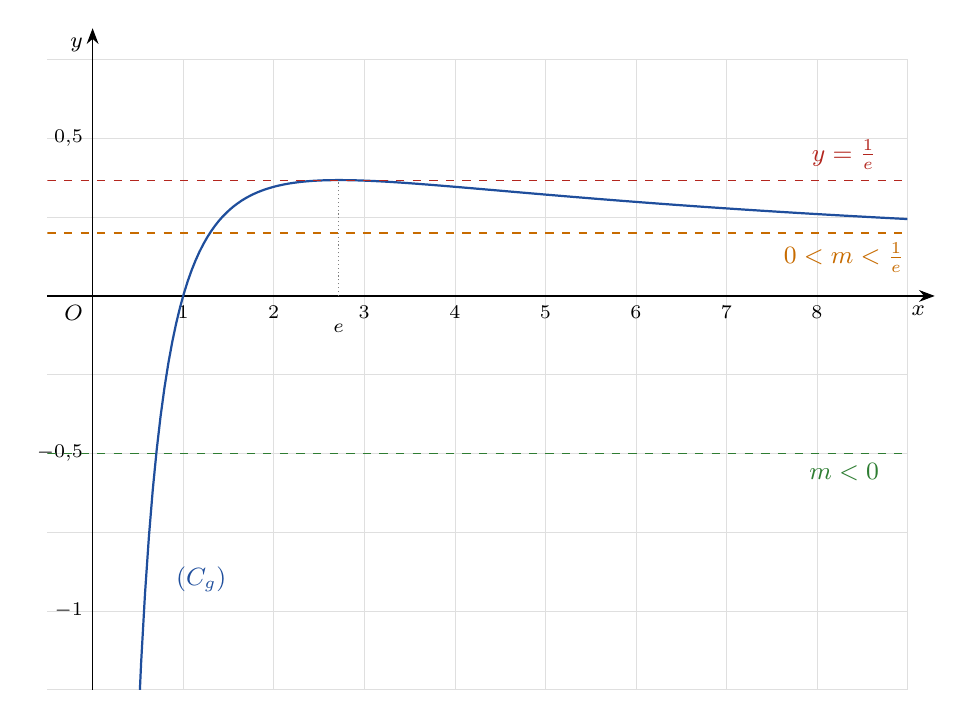
\begin{tikzpicture}[x=1.15cm,y=4cm,font=\footnotesize]
 \draw[gray!25,very thin,xstep=1,ystep=0.25] (-0.5,-1.25) grid (9,0.75);
 \draw[-{Stealth[length=2mm]}] (-0.5,0)--(9.3,0) node[below left]{$x$};
 \draw[-{Stealth[length=2mm]}] (0,-1.25)--(0,0.85) node[below left]{$y$};
 \node[below left] at (0,0){$O$};
 \foreach \t in {1,2,3,4,5,6,7,8} \node[below,font=\scriptsize] at (\t,0){$\t$};
 \foreach \t/\l in {-1/-1,-0.5/-0{,}5,0.5/0{,}5} \node[left,font=\scriptsize] at (0,\t){$\l$};
 \begin{scope}\clip (-0.5,-1.25) rectangle (9,0.75);
 \draw[thick,cDef,domain=0.45:9,samples=200] plot (\x,{ln(\x)/\x});
 \draw[cThm,dashed] (-0.5,0.3679)--(9,0.3679);
 \draw[cEx,dashed] (-0.5,0.2)--(9,0.2);
 \draw[cRem,dashed] (-0.5,-0.5)--(9,-0.5);
 \draw[gray,densely dotted] (2.718,0)--(2.718,0.3679);
 \end{scope}
 \node[cThm,above] at (8.3,0.37) {\small $y=\frac1e$};
 \node[cEx,below] at (8.3,0.2) {\small $0<m<\frac1e$};
 \node[cRem,below] at (8.3,-0.5) {\small $m<0$};
 \node[below,font=\scriptsize] at (2.718,-0.06) {$e$};
 \node[cDef] at (1.2,-0.9) {\small $(C_g)$};
\end{tikzpicture}\end{LTR}\end{center}

\QQ{5}
\pa من أجل $x>0$ (أي $x\neq0$)، بقسمة الطرفين على $x$: $\ln x=mx\iff\dfrac{\ln x}{x}=m\iff g(x)=m$.
إذن حلول المعادلة هي فواصل نقط تقاطع $(C_g)$ مع المستقيم الأفقي $(\Delta_m)$ ذي المعادلة $y=m$.

\pb بالاعتماد على جدول التغيّرات والرسم:
\begin{itemize}
\item إذا كان $m<0$: $(\Delta_m)$ يقطع $(C_g)$ في نقطة واحدة فاصلتها من $]0;1[$: \textbf{حل وحيد}.
\item إذا كان $m=0$: \textbf{حل وحيد  $x=1$}.
\item إذا كان $0<m<\frac1e$: نقطتا تقاطع، فاصلة الأولى من $]1;e[$ والثانية من $]e;+\infty[$: \textbf{حلان}.
\item إذا كان $m=\frac1e$: $(\Delta_m)$ مماس لـ $(C_g)$ عند ذروته: \textbf{حل وحيد  $x=e$}.
\item إذا كان $m>\frac1e$: لا تقاطع: \textbf{لا توجد حلول}.
\end{itemize}

\QQ{6}
\pa من جدول التغيّرات، $\frac1e$ قيمة حدية عظمى للدالة $g$ على $]0;+\infty[$، إذن من أجل كل $x>0$: $\dfrac{\ln x}{x}\leqslant\dfrac1e$، وبضرب الطرفين في $x>0$: $\bx{\ln x\leqslant\dfrac{x}{e}}$.

\pb $\pi\neq e$، والقيمة العظمى $\frac1e$ لا تُبلغ إلا عند $e$، إذن $g(\pi)<\dfrac1e$، أي $\dfrac{\ln\pi}{\pi}<\dfrac{1}{e}$.
بضرب الطرفين في العدد الموجب $e\pi$: $e\ln\pi<\pi$، أي $\ln\left(\pi^{e}\right)<\ln\left(e^{\pi}\right)$.
وبما أن الدالة $\exp$ متزايدة تماما: $\bx{\pi^{e}<e^{\pi}}$. (للتحقق: $\pi^{e}\approx22{,}46$ و $e^{\pi}\approx23{,}14$.)
\end{hal}

% ===================== وجود ووحدانية وحصر α =====================
\begin{tamrin}{وجود وحصر العدد $\alpha$ ونقطة صامدة -- شعبة رياضيات}
\textbf{I)} نعتبر الدالة $g$ المعرفة على $]0;+\infty[$ بـ: $g(x)=x+\ln x-2$.
\QQ{1} أحسب $\lim\limits_{x\to 0^{+}}g(x)$ و $\lim\limits_{x\to +\infty}g(x)$، ثم أدرس اتجاه تغيّر $g$ وشكّل جدول تغيّراتها.
\QQ{2}
\begin{sq}
\qa بيّن أن المعادلة $g(x)=0$ تقبل حلا وحيدا $\alpha$ في $]0;+\infty[$، وأن $1{,}5<\alpha<1{,}6$.
\qb تحقق أن $1{,}55<\alpha<1{,}56$.
\end{sq}
\QQ{3} استنتج إشارة $g(x)$ حسب قيم $x$.

\textbf{II)} نعتبر الدالة $f$ المعرفة على $]0;+\infty[$ بـ: $f(x)=x-2\ln x+\dfrac{1}{2}(\ln x)^{2}$.
\QQ{1} أحسب $\lim\limits_{x\to 0^{+}}f(x)$، ثم بيّن أنه من أجل كل $x>0$: $f(x)\geqslant x-2\ln x$ واستنتج $\lim\limits_{x\to +\infty}f(x)$.
\QQ{2} بيّن أنه من أجل كل عدد حقيقي $x$ من $]0;+\infty[$: $f'(x)=\dfrac{g(x)}{x}$، ثم شكّل جدول تغيّرات $f$.
\QQ{3}
\begin{sq}
\qa بيّن أن $f(\alpha)=\dfrac{\alpha^{2}}{2}+\alpha-2$.
\qb استنتج حصرا للعدد $f(\alpha)$، ثم بيّن أنه من أجل كل $x>0$: $f(x)>0$.
\end{sq}

\textbf{III)} نعتبر الدالة $\varphi$ المعرفة على $]0;+\infty[$ بـ: $\varphi(x)=2-\ln x$، و $(\Delta)$ المستقيم ذو المعادلة $y=x$.
\QQ{1} بيّن أن $\alpha$ هو الحل الوحيد للمعادلة $\varphi(x)=x$ (نقول إن $\alpha$ نقطة صامدة للدالة $\varphi$).
\QQ{2} أدرس الوضع النسبي للمنحنى $(C_\varphi)$ والمستقيم $(\Delta)$.
\QQ{3}
\begin{sq}
\qa بيّن أنه إذا كان $x\in[1{,}5;1{,}6]$ فإن $\varphi(x)\in[1{,}5;1{,}6]$.
\qb باستعمال $\varphi(\alpha)=\alpha$ والحصر $1{,}55<\alpha<1{,}56$، بيّن أن $1{,}555<\alpha<1{,}56$.
\end{sq}
\QQ{4} ارسم $(\Delta)$ و $(C_\varphi)$ في معلم متعامد ومتجانس.
\end{tamrin}

\begin{hal}
\textbf{الجزء I}
\QQ{1} $\lim\limits_{x\to0^{+}}\ln x=-\infty$ إذن $\bx{\lim\limits_{x\to0^{+}}g(x)=-\infty}$، و $\lim\limits_{x\to+\infty}(x-2)=\lim\limits_{x\to+\infty}\ln x=+\infty$ إذن $\bx{\lim\limits_{x\to+\infty}g(x)=+\infty}$.
$g$ قابلة للاشتقاق على $]0;+\infty[$ ومن أجل كل $x>0$: $g'(x)=1+\dfrac1x>0$. إذن $g$ \textbf{متزايدة تماما} على $]0;+\infty[$.
\begin{TAB}
\tkzTabInit[lgt=2,espcl=5]{$x$/0.8,$g'(x)$/0.8,$g(x)$/1.6}{$0$,$+\infty$}
\tkzTabLine{d,+,}
\tkzTabVar{D-/$-\infty$,+/$+\infty$}
\end{TAB}

\QQ{2}
\pa الدالة $g$ مستمرة ومتزايدة تماما على $]0;+\infty[$، وتأخذ قيمها في $]-\infty;+\infty[$ الذي يشمل $0$؛ إذن حسب مبرهنة القيم المتوسطة (حالة الرتابة التامة) المعادلة $g(x)=0$ تقبل حلا وحيدا $\alpha$.
ولدينا: $g(1{,}5)=-0{,}5+\ln1{,}5\approx-0{,}095<0$ و $g(1{,}6)=-0{,}4+\ln1{,}6\approx0{,}070>0$.
بما أن $g(1{,}5)\times g(1{,}6)<0$ و $g$ مستمرة ومتزايدة تماما على $[1{,}5;1{,}6]$: $\bx{1{,}5<\alpha<1{,}6}$.

\pb $g(1{,}55)\approx-0{,}0117<0$ و $g(1{,}56)\approx0{,}0047>0$، إذن بنفس الطريقة: $\bx{1{,}55<\alpha<1{,}56}$.

\QQ{3} بما أن $g$ متزايدة تماما و $g(\alpha)=0$:
من أجل $x\in]0;\alpha[$: $\bx{g(x)<0}$، ومن أجل $x\in]\alpha;+\infty[$: $\bx{g(x)>0}$، و $g(\alpha)=0$.

\textbf{الجزء II}
\QQ{1} \textbf{عند $0^{+}$:} نكتب $f(x)=x+\ln x\left(\dfrac12\ln x-2\right)$.
لما $x\to0^{+}$: $\ln x\to-\infty$ و $\dfrac12\ln x-2\to-\infty$، فجداؤهما يؤول إلى $+\infty$، ومنه $\bx{\lim\limits_{x\to0^{+}}f(x)=+\infty}$.

\textbf{عند $+\infty$:} من أجل كل $x>0$: $\dfrac12(\ln x)^{2}\geqslant0$، إذن $\bx{f(x)\geqslant x-2\ln x}$.
ولدينا $x-2\ln x=x\left(1-2\,\dfrac{\ln x}{x}\right)$ و $\lim\limits_{x\to+\infty}\dfrac{\ln x}{x}=0$، إذن $\lim\limits_{x\to+\infty}(x-2\ln x)=+\infty$.
وحسب مبرهنة المقارنة: $\bx{\lim\limits_{x\to+\infty}f(x)=+\infty}$.

\QQ{2} $f$ قابلة للاشتقاق على $]0;+\infty[$، ولدينا $\left((\ln x)^{2}\right)'=\dfrac{2\ln x}{x}$؛ إذن من أجل كل عدد حقيقي $x$ من $]0;+\infty[$:
\[f'(x)=1-\frac{2}{x}+\frac12\times\frac{2\ln x}{x}=\frac{x-2+\ln x}{x}=\bx{\frac{g(x)}{x}}\]
بما أن $x>0$، إشارة $f'(x)$ هي إشارة $g(x)$: $f$ متناقصة تماما على $]0;\alpha]$ ومتزايدة تماما على $[\alpha;+\infty[$.
\begin{TAB}
\tkzTabInit[lgt=2,espcl=3.5]{$x$/0.8,$f'(x)$/0.8,$f(x)$/1.6}{$0$,$\alpha$,$+\infty$}
\tkzTabLine{d,-,z,+,}
\tkzTabVar{D+/$+\infty$,-/$f(\alpha)$,+/$+\infty$}
\end{TAB}

\QQ{3}
\pa لدينا $g(\alpha)=0$، أي $\alpha+\ln\alpha-2=0$، ومنه $\ln\alpha=2-\alpha$. بالتعويض:
\begin{align*}
f(\alpha)&=\alpha-2(2-\alpha)+\frac12(2-\alpha)^{2}=\alpha-4+2\alpha+\frac12\left(4-4\alpha+\alpha^{2}\right)\\
&=3\alpha-4+2-2\alpha+\frac{\alpha^{2}}{2}=\bx{\frac{\alpha^{2}}{2}+\alpha-2}
\end{align*}
\pb الدالة $u:t\mapsto\dfrac{t^{2}}{2}+t-2$ متزايدة تماما على $]0;+\infty[$ (لأن $u'(t)=t+1>0$). من $1{,}55<\alpha<1{,}56$ نستنتج $u(1{,}55)<f(\alpha)<u(1{,}56)$:
\[\bx{0{,}751<f(\alpha)<0{,}777}\]
(لأن $u(1{,}55)=0{,}75125$ و $u(1{,}56)=0{,}7768$.)
$f(\alpha)$ هي القيمة الحدية الصغرى للدالة $f$ على $]0;+\infty[$، وهي موجبة تماما، إذن من أجل كل $x>0$: $f(x)\geqslant f(\alpha)>0$، أي $\bx{f(x)>0}$.

\textbf{الجزء III}
\QQ{1} من أجل $x>0$: $\varphi(x)=x\iff 2-\ln x=x\iff x+\ln x-2=0\iff g(x)=0$.
وحسب الجزء I هذه المعادلة تقبل حلا وحيدا هو $\alpha$. إذن $\bx{\varphi(\alpha)=\alpha}$ و $\alpha$ هو النقطة الصامدة الوحيدة للدالة $\varphi$.

\QQ{2} من أجل $x>0$: $\varphi(x)-x=2-\ln x-x=-g(x)$. إذن:
\begin{FIG}
\begin{tikzpicture}[font=\normalsize]
\fill[gray!12] (0,0) rectangle (2.6,-0.9);
\fill[green!18] (2.6,0) rectangle (15.5,-0.9);
\fill[orange!45] (0,-0.9) rectangle (2.6,-4.6);
\fill[cyan!22] (2.6,-0.9) rectangle (15.5,-4.6);
\draw[thick] (0,0) rectangle (15.5,-4.6); \draw (0,-0.9)--(15.5,-0.9) (0,-1.8)--(15.5,-1.8) (2.6,0)--(2.6,-4.6);
\node at (1.3,-0.45){$x$};
\node at (1.3,-1.35){$\varphi(x)-x$};
\node[align=center,font=\bfseries] at (1.3,-3.2){\ar{الوضع}\\ \ar{النسبي}};
\node at (3.3,-0.45){$0$};
\node at (9.05,-0.45){$\alpha$};
\node at (14.8,-0.45){$+\infty$};
\node at (5.425,-1.35){$+$};
\node[align=center,font=\small] at (5.425,-3.2){$(C_\varphi)$\\ \ar{فوق}\\ $(\Delta)$};
\node at (12.675,-1.35){$-$};
\node[align=center,font=\small] at (12.675,-3.2){$(C_\varphi)$\\ \ar{تحت}\\ $(\Delta)$};
\draw[double,thick] (3.3,-0.9)--(3.3,-4.6);
\node at (9.05,-1.35){$0$};
\draw[densely dotted] (9.05,-0.9)--(9.05,-1.13) (9.05,-1.57)--(9.05,-1.8);
\draw (7.55,-4.6) .. controls (7.625,-3.06) and (8.6,-2.136) .. (9.05,-1.8) .. controls (9.5,-2.136) and (10.475,-3.06) .. (10.55,-4.6);
\node[align=center,font=\footnotesize,inner sep=0pt] at (9.05,-3.65){\ar{$(C_\varphi)$ يقطع}\\ $(\Delta)$\\ \ar{في النقطة}\\ $B(\alpha;\alpha)$};
\end{tikzpicture}
\end{FIG}

\QQ{3}
\pa $\varphi'(x)=-\dfrac1x<0$، إذن $\varphi$ متناقصة تماما على $[1{,}5;1{,}6]$. فإذا كان $1{,}5\leqslant x\leqslant1{,}6$ فإن $\varphi(1{,}6)\leqslant\varphi(x)\leqslant\varphi(1{,}5)$.
ولدينا $\varphi(1{,}6)=2-\ln1{,}6\approx1{,}530$ و $\varphi(1{,}5)=2-\ln1{,}5\approx1{,}595$، إذن $1{,}5<1{,}530\leqslant\varphi(x)\leqslant1{,}595<1{,}6$، أي $\bx{\varphi(x)\in[1{,}5;1{,}6]}$.

\pb من $1{,}55<\alpha<1{,}56$ و $\varphi$ متناقصة تماما: $\varphi(1{,}56)<\varphi(\alpha)<\varphi(1{,}55)$.
لكن $\varphi(\alpha)=\alpha$، و $\varphi(1{,}56)=2-\ln1{,}56\approx1{,}5553$ و $\varphi(1{,}55)\approx1{,}5617$، إذن $1{,}5553<\alpha<1{,}5617$.
وبأخذ تقاطع هذا الحصر مع $1{,}55<\alpha<1{,}56$ نجد $\bx{1{,}555<\alpha<1{,}56}$ (وهذا حصر سعته $0{,}005$؛ القيمة الفعلية $\alpha\approx1{,}557$).

\QQ{4} نقاط مساعدة: $\varphi(1)=2$؛ $\varphi(e)=1$؛ $\varphi\left(e^{2}\right)=0$ أي $(C_\varphi)$ يقطع محور الفواصل عند $e^{2}\approx7{,}39$؛ $\lim\limits_{x\to0^{+}}\varphi(x)=+\infty$ و $\lim\limits_{x\to+\infty}\varphi(x)=-\infty$.
\begin{GR}{-0.5}{8}{-1}{4.5}{1.1}
\Ticks{1,2,3,4,5,6,7}{-1,1,2,3,4}
\draw[thick,cDef,domain=0.09:8,samples=200] plot (\x,{2-ln(\x)});
\draw[thick,cThm] (-0.5,-0.5)--(4.5,4.5);
\fill (1.5571,1.5571) circle (1.6pt) node[above left]{$B$};
\draw[gray,densely dotted] (1.5571,0)--(1.5571,1.5571);
\node[below] at (1.5571,-0.25) {\scriptsize $\alpha$};
\node[cDef] at (6,0.6) {\small $(C_\varphi)$};
\node[cThm] at (4,4.4) {\small $(\Delta)$};
\end{GR}
\end{hal}

\end{document}
